%---------------------------------------------------------------------------------
%	CHAPTER FILE (C.Stamper template)
%---------------------------------------------------------------------------------

%\onehalfspace
\chapter[Low-Reynolds number gravitational settling of a sphere through a fluid-fluid interface: A boundary integral model]{Low-Reynolds number gravitational settling of a sphere through a fluid-fluid interface: A boundary integral model}
\chaptermark{Boundary integral model}
\label{ch:mod} % label for referring to chapter in other parts of the thesis
\textbf{ABSTRACT}\\
\small{Chapter abstract} % Having a chapter abstract is optional
\vfill
\small{\textbf{Author Contributions:} Detail who did what.
\newpage

\section{Introduction}
\label{sec:intro}


\section{Fundamentals of Stokes Flow}
\label{sec:Stokes}

Presented here is a background to the fundamentals of Stokes flow, covering the equations of motion and non-dimensionalisation, different types of boundary condition, Greens functions and the integral representation of Stokes flow. The Einstein summation convention and tensor notation \citep{Riley06} will be used throughout.

\begin{comment}
    \begin{longtable}{|c|c|}
    \caption{Definition of symbols. \label{tab:symbols}} \\ % title name of the table
    \hline
    Symbol & Definition \\  
    \hline % inserts single-line
    $a$                                                                           & Sphere radius           \\
    $\mathrm{e}$                                                                  & Exponential constant \\
    $\hat{e}_{\alpha,ij}$                                                           & Greens function for strain in fluid $\alpha$ \\
    $f_{\text{s},i}(\boldsymbol{x}) = m_{j}(\boldsymbol{x})T_{1,ij}(\boldsymbol{x})$   &Traction on surface of sphere \\
    $f_{\alpha,i}(\boldsymbol{x}) = n_{j}(\boldsymbol{x})T_{\alpha,ij}(\boldsymbol{x})$ & Traction of fluid $\alpha$ on interface \\
    $\mathcal{F}_{i}$                                                              & Arbitrary constant vector \\
    $\boldsymbol{F}$                                                              & Force vector \\
    $\boldsymbol{g} = (-9.81 \text{m s}^{-2}) \boldsymbol{\hat{z}}$                & Acceleration due to gravity \\      
    $\mathcal{I}$                                                                 & Surface of interface \\
    $i = \sqrt{-1}$                                                               & The unit imaginary number \\
    $J_{ij}$                                                                       & Components of tensor kernel for velocity Greens function \\
    $K_{ijk}$                                                                     & Components of tensor kernel for stress Greens function \\
    $\boldsymbol{k}$                                                              & Dummy variable in Fourier space \\
    $k = |\boldsymbol{k}|$                                                        & Magnitude of $\boldsymbol{k}$ \\
    $m$                                                                           & Outward normal to sphere surface \\
    $n$                                                                           & Normal to interface (points into fluid 1) \\
    $P_{\alpha}(\boldsymbol{x})$                                                    & Pressure field of fluid $\alpha$ \\
    $P_{\text{d},\alpha}(\boldsymbol{x}) $                                            & Dynamic pressure of fluid $\alpha$ \\
    $\hat{P}_{\alpha}$                                                       & Greens function for dynamic pressure of fluid $\alpha$ \\
    $\bar{P}_{\alpha, i}(\boldsymbol{\xi})$                                            & Components of the vector of solutions for $\hat{P}_{\alpha}$ in equation~\ref{equ:stokes_green} \\
    $\tilde{P}_{\alpha, i} (\boldsymbol{k})$                                         & Fourier transform of $\bar{P}_{\alpha, i}(\boldsymbol{\xi})$ \\
    $s$                                                                           & Arc length along interface measured from axis \\
    $\mathcal{S}$                                                                 & Surface of sphere \\
    $T_{\alpha,ij}(\boldsymbol{x})$                                                  & Stress tensor field of fluid $\alpha$ \\
    $\hat{T}_{\alpha,ij}(\boldsymbol{x'} - \boldsymbol{y'})$                         & Stress Greens function for fluid $\alpha$ \\
    $t$                                                                           & Time \\
    $\boldsymbol{u}_{\alpha}(\boldsymbol{x})$                                       & Velocity field of fluid $\alpha$ \\
    $\boldsymbol{u}_{\text{s}} = u_{\text{s}} \boldsymbol{\hat{z}}$                    & Velocity of sphere \\
    $\hat{u}_{\alpha,i}(\boldsymbol{x'} - \boldsymbol{y'})$                         & Velocity Greens function for fluid $\alpha$ \\
    $\bar{u}_{\alpha, i,j}(\boldsymbol{\xi})$                                        & Components of the tensor of solutions for $\hat{u}_{\alpha,i}$ in equation~\ref{equ:stokes_green} \\
    $\tilde{u}_{\alpha, ij}(\boldsymbol{k})$                                         & Fourier transform of $\bar{u}_{\alpha, i,j}(\boldsymbol{\xi})$ \\
    $\mathcal{V}_{\alpha}$                                                          & Volume of fluid $\alpha$ \\
    $\boldsymbol{x}$                                                              & Position vector \\
    $\boldsymbol{y}$                                                              & Position vector \\
    $\boldsymbol{\hat{z}}$                                                        & Unit vector in the upward vertical direction \\
    $\alpha = 1,2$                                                                & Fluid label \\
    $\delta_{ij} = \begin{cases}
    1  & \quad \text{if } i = j\\
    0  & \quad \text{if } i \neq j\\
  \end{cases}$                                                                    & Kronecker delta \\
    $\delta(\boldsymbol{x'} - \boldsymbol{y'}) = \begin{cases}
    1  & \quad \text{if } \boldsymbol{x} = \boldsymbol{y}\\
    0  & \quad \text{if } \boldsymbol{x} \neq \boldsymbol{y}\\
  \end{cases}$                                                                    & Dirac delta function \\
    $\eta_{\alpha}$                                                                 & Viscosity of fluid $\alpha$ \\ 
    $\theta$                                                                      & Polar angle with respect to sphere centre \\
    $\rho_{\alpha}$                                                                 & Density of fluid $\alpha$   \\
    $\rho_{\text{s}}$                                                                & Sphere density          \\
    $\sigma$                                                                      & Interfacial Tension     \\
    $\phi$                                                                        & Azimuhtal angle with respect to axis of motion \\
    $\boldsymbol{\xi} = \boldsymbol{x'} - \boldsymbol{y'}$                        & Dimensionless separation vector \\                                   
    $\xi = |\boldsymbol{\xi}|$                                                    & Magnitude of $\boldsymbol{\xi}$ \\
    \hline % inserts single-line
  \end{longtable}
\end{comment}

\subsection{Equations of Motion}
\label{subsec:EoM}

The starting points for the majority of fluid dynamical problems are the continuity (equation~\ref{equ:full_cont}) and Navier Stokes (equation~\ref{equ:NS_comp}) equations \citep{Batchelor67}. Defining the fluid density $\rho$, the dynamic viscosity $\eta$, the fluid velocity field $u_{i}$, the pressure field $P$ and the acceleration due to gravity as $g = 9.81$ m s$^{-2}$, these are expressed as

\begin{equation}
\label{equ:full_cont}
\frac{\partial \rho(\boldsymbol x,t)}{\partial t} + \partial_{i} [\rho(\boldsymbol{x},t) u_{i} (\boldsymbol{x},t)] = 0 ,
\end{equation}  

and 

\begin{align}
\label{equ:NS_comp}
\left( \frac{\partial [u_{i}(\boldsymbol{x},t) \rho(\boldsymbol{x},t)]}{\partial t} + u_{j}(\boldsymbol{x},t) \partial_{j} [u_{i}(\boldsymbol{x},t) \rho(\boldsymbol{x},t)] \right) = - \partial_{i} P(\boldsymbol{x},t) - \rho(\boldsymbol{x},t) g + \nonumber \\ 
\eta \left(\partial_{j} \partial_{j} u_{i}(\boldsymbol{x},t) + \frac{\partial_{i} (\partial_{j} u_{j}(\boldsymbol{x},t))}{3} \right).
\end{align} 

Forming a coupled set of non-linear, partial differential equations for the velocity and pressure fields as functions of space $\boldsymbol{x}$ and time $t$, these represent mass and momentum conservation respectively, and must be satisfied by all Newtonian fluid phases within the system. For many practical applications, including magmatic melt, the fluids are assumed to be incompressible (have constant density) and so the continuity equation reduces to the incompressibility relation,

\begin{equation}
\label{equ:incom}
\partial_{i} u_{i}(\boldsymbol{x},t) = 0 .
\end{equation}

This can be combined with equation~\ref{equ:NS_comp} to give the incompressible Navier Stokes equation,

\begin{equation}
\label{equ:NS_incom}
\rho \left( \frac{\partial u_{i}(\boldsymbol{x},t)}{\partial t} + u_{j}(\boldsymbol{x},t) \partial_{j} u_{i}(\boldsymbol{x},t) \right) = - \partial_{i} P(\boldsymbol{x},t) - \rho g + \eta \partial_{j} \partial_{j} u_{i}(\boldsymbol{x},t) .
\end{equation} 

The equations of motion can be expressed in an alternative form by defining the stress tensor $T_{ij}(\boldsymbol{x},t)$ \citep{Batchelor67, Manga94} and dynamic pressure $P_{\text{d}}(\boldsymbol{x},t)$:

\begin{equation}
\label{equ:stress}
T_{ij}(\boldsymbol{x},t) = -P_{\text{d}}(\boldsymbol{x},t)  \delta_{ij} + \eta[\partial_{i} u_{j}(\boldsymbol{x},t) + \partial_{j} u_{i}(\boldsymbol{x},t)], 
\end{equation}

and 

\begin{equation}
\label{equ:dyn_P}
P_{\text{d}}(\boldsymbol{x},t) = P(\boldsymbol{x},t) - \rho g_{i} x_{i} ,
\end{equation}

where $\delta_{ij}$ are the components of the Kronecker delta tensor \citep{Riley06}. This definition of the stress tensor removes the explicit appearence of the gravitational body force from the equations of motion, meaning they only appears in the boundary conditions. The Navier Stokes equation then becomes

\begin{equation}
\label{equ:NS_stress}
\rho \left( \frac{\partial u_{i}(\boldsymbol{x},t)}{\partial t} + [u_{j}(\boldsymbol{x},t) \partial_{j}] u_{i}(\boldsymbol{x},t) \right) = \partial_{j} T_{ij}(\boldsymbol{x},t) .
\end{equation}

When working in fluid dynamics, it is usual to non-dimensionalise the equations of motion and boundary conditions \citep{White99}. This can be achieved by scaling the quantities involved by parameters specific to the problem. For example, consider a problem with typical scales of length $L_{\text{c}}$ and velocity $U_{\text{c}}$. This allows dimensionless variables (denoted by a $'$) to be defined:

\begin{equation} 
\label{equ:nodim_l}
x_{i} = L_{\text{c}} x'_{i} ,
\end{equation}

\begin{equation}
\label{equ:nodim_u}
u_{i}(\boldsymbol{x},t) = U_{\text{c}} u'_{i}(\boldsymbol{x'},t') ,
\end{equation}

and 

\begin{equation}
\label{equ:nodim_t}
t = \frac{L_{\text{c}} t'}{U_{\text{c}}}.
\end{equation}

In the case of highly viscous flows the relevant scaling for the dynamic pressure uses a characteristic viscosity $\eta_{\text{c}}$ and is given by \citep{Lee82}

\begin{equation}
\label{equ:nodim_p_highRE}
P_{\text{d}}(\boldsymbol{x},t) = \frac{\eta_{\text{c}} U_{\text{c}} P_{\text{d}}'(\boldsymbol{x'},t')}{L_{\text{c}}} .
\end{equation}

This choice of pressure scaling means that upon substitution of equations~\ref{equ:nodim_l} to~\ref{equ:nodim_p_highRE} into equation~\ref{equ:stress}, the stress tensor can also be non-dimensionalised,

\begin{equation}
\label{equ:nodim_T}
T_{ij}(\boldsymbol{x},t) = \frac{\eta_{\text{c}} U_{\text{c}} T'_{ij}(\boldsymbol{x'},t')}{L_{\text{c}}}, \quad \text{where} \quad T'_{ij}(\boldsymbol{x'},t') = P_{\text{d}}'(\boldsymbol{x'},t') \delta_{ij} + \Lambda [\partial'_{i} u'_{j}(\boldsymbol{x'},t') + \partial'_{j} u'_{i}(\boldsymbol{x'},t')] ,
\end{equation}

where $\Lambda = \eta / \eta_{\text{c}}$. Hence, the dimensionless continuity and Navier Stokes equations are

\begin{equation}
\label{equ:nodim_cont}
\partial'_{i} u'_{i}(\boldsymbol{x'},t') = 0,
\end{equation}

and

\begin{equation}
\label{equ:NS_low_Reynolds}
\Rey \left(\frac{\partial u'_{i}(\boldsymbol{x'},t')}{\partial t'} + u'_{j}(\boldsymbol{x'},t' \partial'_{j}) u'_{i}(\boldsymbol{x'},t') \right) = \partial'_{j} T'_{ij}(\boldsymbol{x'},t') ,
\end{equation}

where the Reynolds number $\Rey$ is defined as

\begin{equation}
\label{equ:Reynolds}
\Rey = \frac{\rho L_{\text{c}} U_{\text{c}}}{\eta_{\text{c}}}.
\end{equation}

As we are considering the case of low Reynolds number ($\text{Re} \ll 1$), we can neglect the inertial terms on the left hand side of equation~\ref{equ:NS_low_Reynolds}, and the equation reduces to the Stokes equation \citep{Batchelor67, Kim05},

\begin{equation}
\label{equ:Stokes}
\partial'_{i} T'_{ij}(\boldsymbol{x'}) = 0 .
\end{equation}

Note that the explicit time dependence has now vanished from the Stokes equations. However, it is still valid to use the equations for time dependent flows, where the boundary conditions change with time, if the quasi-static assumption is satisfied;

\begin{equation}
\label{equ:quasi_stat}
\frac{L_{\text{c}}^{2} \rho}{\eta_{\text{c}}} \ll \tau
\end{equation}

where $\tau$ is a typical timescale for a change in flow geometry. Physically, this means that the velocity and stress fields of the fluid respond instantaneously to changes in the boundary conditions \citep{Manga94}.

\subsection{Boundary Conditions}
\label{subsec:BC}

In order to complete the formulation of any fluid dynamics problem, it is necessary to state the boundary conditions alongside the equations of motion \citep{Riley06}. For fluids of infinite (or semi-infinite) extent in some dimension, these include the flow velocity at infinity. For bounded flows, the conditions are imposed at the boundaries of the fluid domain, and their exact nature depends on the phase of the material bounding it. At a boundary, two types of boundary condition can exist: a kinematic boundary condition on the velocity field and a dynamic boundary condition on the stress field (derivative of the velocity field). Kinematic boundary conditions are an expression of mass conservation and dynamic boundary conditions are a balance of forces (effectively an expression of Newton's third law). Geometric symmetries can be exploited to identify further boundary conditions and reduce the complexity of problems. In unsteady flows, initial conditions are also important, but since this work considers quasi-static flows, they will not be discussed here.

\subsubsection{Fluid-Solid Boundary}
\label{subsubsec:BC_fluid-solid}

At low Reynolds number, for a fluid-solid boundary defined the by surface $\mathcal{S}$ (see figure~\ref{fig:fluid-solid_boundary}), the kinematic boundary condition usually employed is one of no-slip; the fluid velocity at the boundary is the same as that of the solid $U'_{\text{s},i}$. This is easily expressed in dimensionless form as

\begin{equation}
\label{equ:lowRE_fluid-solid}
u'_{i}(\boldsymbol{x'}) = U_{\text{s}, i}', \quad \text{for }\boldsymbol{x} \in \mathcal{S} .
\end{equation}


\begin{figure}
$$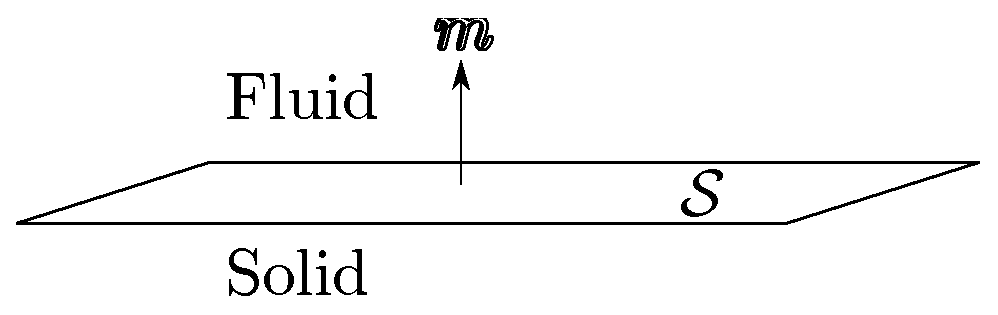
\includegraphics[width=80mm]{../../Programming/sinking_bim_write_up/trunk/fluid_solid.eps}$$
\caption{Fluid-solid boundary $\mathcal{S}$ with normal vector $\boldsymbol{m}$ directed into the fluid phase. \label{fig:fluid-solid_boundary}}
\end{figure}

This is valid for situations where the fluid domain is much larger than the mean free path of molecules within the fluid. If this isn't true, a slip condition can be employed at the boundary \citep{Dussan76}. There also needs to be a dynamic boundary condition applied at the interface. If the solid exerts a force $F_{i}$ onto the fluid, then the condition states

\begin{equation}
\label{equ:dyn_fluid_solid}
\int_{\mathcal{S}} m_{i}(\boldsymbol{x}) T_{ij}(\boldsymbol{x}) \mathrm{d} \mathcal{S} = F_{j} ,
\end{equation}

where $m_{i}(\boldsymbol{x})$ is the normal vector to $\mathcal{S}$ directed into the fluid. Using the non-dimensionalisation scheme presented above this becomes

\begin{equation}
\label{equ:nodim_fluid_solid}
\eta_{\text{c}} U_{\text{c}} L_{\text{c}} \int_{\mathcal{S}} f_{i}(\boldsymbol{x'}) \mathrm{d} \mathcal{S'} = F_{i} ,
\end{equation}

where $f_{i}(\boldsymbol{x'}) =m_{i}(\boldsymbol{x'}) T'_{ij}(\boldsymbol{x'})$ is defined as the dimensionless traction vector on the surface $\mathcal{S}$.

\subsubsection{Fluid-Fluid Boundary}
\label{subsubsec:BC_fluid-fluid}

For a boundary $\mathcal{I}$ between two fluids labelled 1 and 2 (figure~\ref{fig:fluid-fluid_boundary}), the usual kinematic boundary condition states that the velocity of the two fluids must be continuous across the interface \citep{Kim05}. Defining the velocity of fluid $l$ as $u_{l}$, this can be expressed in dimensionless form as

\begin{equation}
\label{equ:fluid_fluid_kin}
u'_{1,i}(\boldsymbol{x'}) = u'_{2,i}(\boldsymbol{x'}), \quad \text{for } \boldsymbol{x'} \in \mathcal{I} .
\end{equation}

\begin{figure}
$$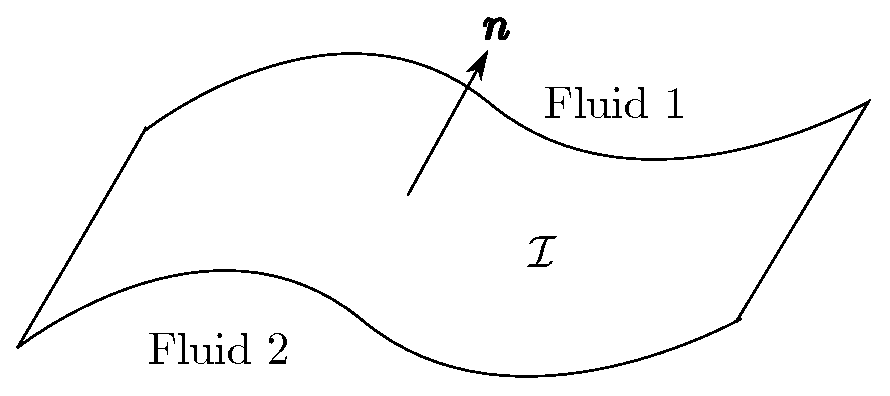
\includegraphics[width=80mm]{../../Programming/sinking_bim_write_up/trunk/fluid_fluid.eps}$$
\caption{Fluid-fluid boundary $\mathcal{I}$ with normal vector $\boldsymbol{n}$. \label{fig:fluid-fluid_boundary}}
\end{figure}

Again, if the fluid domains are small compared to the mean free path of molecules, a slip condition can be employed instead \citep{Maxwell1879}. The dynamic boundary condition is an expression of the balance between the stress discontinuity across the interface and the interfacial tension (IFT) $\sigma$ \citep{Batchelor67}. With the stress tensor defined by equation~\ref{equ:stress}, this is given by \citep{Manga94}

\begin{align}
\label{equ:fluid_fluid_dyn}
n_{i}(\boldsymbol{x}) [T_{1,ij}(\boldsymbol{x}) - \rho_{1} g x_{z} \delta_{ij}] - n_{i}(\boldsymbol{x}) [T_{2,ij}(\boldsymbol{x}) - \rho_{2} g x_{z} \delta_{ij}] = \\ \nonumber
\sigma(\boldsymbol{x}) n_{j}(\boldsymbol{x}) [\partial_{\text{s},i} n_{i}(\boldsymbol{x})] - \partial_{\text{s},j} \sigma (\boldsymbol{x}) , \quad \text{for } \boldsymbol{x} \in \mathcal{I} ,
\end{align}

where $n_{i}$ is the normal vector to the surface $\mathcal{I}$ directed into fluid 1 and $x_{z}$ is the vertical position of the point $\boldsymbol{x}$. The operator $\partial_{\text{s},i}$ is defined as the tangential gradient operator within the surface $\mathcal{I}$:

\begin{equation}
\label{equ:surf_grad}
\partial_{\text{s},i} = (\delta_{ij} - \partial_{i} \partial_{j}) \partial_{j} .
\end{equation}

If this takes the normal vector as its argument it can be shown that \citep{Brackbill92}

\begin{equation}
\label{equ:tang_diff_norm}
\partial_{\text{s},i} n_{i}(\boldsymbol{x}) = \partial_{i} n_{i}(\boldsymbol{x}).
\end{equation}

The presence of spatial gradients in the interfacial tension can lead to so-called Marangoni effects \citep{Thomson1855, Gibbs1878}. However, for these purposes it is assumed that the interfacial tension is uniform across the interface $\mathcal{I}$, and so the last term on the right hand side vanishes,

\begin{align}
\label{equ:fluid_fluid_dyn_nograd}
n_{i}(\boldsymbol{x}) [{T}_{1,ij} (\boldsymbol{x}) - \rho_{1} g x_{z} \delta_{ij}] - n_{i}(\boldsymbol{x}) [T_{2,ij}(\boldsymbol{x}) - \rho_{2} g x_{z} \delta_{ij}] = \\ \nonumber
\sigma(\boldsymbol{x}) n_{i}(\boldsymbol{x}) \partial_{i} n_{j}(\boldsymbol{x}),  \quad \text{for }\boldsymbol{x} \in \mathcal{I}.
\end{align}

Like the equations of motion, this can be non-dimensionalised using equations~\ref{equ:nodim_l} to~\ref{equ:nodim_T}

\begin{equation}
\label{equ:nodim_fluid_fluid_dyn}
n_{i}(\boldsymbol{x'}) [T'_{1,ij}(\boldsymbol{x'}) - T'_{2,ij}(\boldsymbol{x'})] \Ca + \Bo x'_{z} n_{j}(\boldsymbol{x'}) = n_{j}(\boldsymbol{x'}) \partial'_{i} n_{i}(\boldsymbol{x'}) \quad \text{for }\boldsymbol{x'} \in \mathcal{I}.
\end{equation}

The capillary number $\Ca$ and  Bond number $\Bo$ are dimensionless numbers defined as:

\begin{equation}
\label{equ:cap}
\Ca = \frac{\eta_{\text{c}} U_{\text{c}}}{\sigma},
\end{equation}

and

\begin{equation}
\label{equ:Bond}
\Bo = \frac{(\rho_{2} - \rho_{1}) g L_{\text{c}}^{2}}{\sigma}.
\end{equation}

\subsection{Greens functions}
\label{subsec:BIE_deriv}

In order to derive the integral representation of the Stokes equations, it is necessary to make use of the Greens functions \citep{Riley06} for Stokes flow, $\hat{u}_{i}(\boldsymbol{x'} - \boldsymbol{y'})$ and $\hat{T}_{ij}(\boldsymbol{x'} - \boldsymbol{y'})$, defined such that \citep{Kim05}

\begin{equation}
\label{equ:vel_green_def}
\partial'_{i} \hat{u}_{i}(\boldsymbol{x'} - \boldsymbol{y'}) = 0,
\end{equation}

and

\begin{equation}
\label{equ:stress_green_def}
\partial'_{i} \hat{T}_{ij}(\boldsymbol{x'} - \boldsymbol{y'}) + \mathcal{F}_{j} \delta(\boldsymbol{x'} - \boldsymbol{y'}) = 0 , 
\end{equation}

where $\mathcal{F}_{i}$ is a arbitrary constant vector, $\delta(\boldsymbol{x'} - \boldsymbol{y'})$ is the Dirac delta-function (appendix~\ref{app:delta}) and both $\hat{u}_{i}(\boldsymbol{x'})$ and $\hat{T}_{ij}(\boldsymbol{x'}) \to 0$ as $|\boldsymbol{x'}| \to \infty$. Equations~\ref{equ:vel_green_def} and~\ref{equ:stress_green_def} can be solved following \citet{Ladyzhenskaya63} showing that (see appendix~\ref{app:Greens})

\begin{equation}
\label{equ:vel_green}
\hat{u}_{j}(\boldsymbol{\xi}) = \frac{ \mathcal{F}_{i} J_{ij}(\boldsymbol{\xi})}{\Lambda} ,
\end{equation}

and 

\begin{equation}
\label{equ:stress_green}
\hat{T}_{ij}(\boldsymbol{\xi}) = K_{ijk}(\boldsymbol{\xi}) \mathcal{F}_{k} ,
\end{equation}

where $\boldsymbol{\xi} = \boldsymbol{x'} - \boldsymbol{y'}$,

\begin{equation}
\label{equ:J_kernal}
J_{ij}(\boldsymbol{\xi}) = \frac{1}{8 \pi \xi} \left( \delta_{ij} + \frac{\xi_{i} \xi_{j}}{\xi^{2}} \right) ,
\end{equation}


\begin{equation}
\label{equ:K_kernal}
K_{ijk}(\boldsymbol{\xi}) = \frac{-3 \xi_{i} \xi_{j} \xi_{k}}{4 \pi \xi^{5}},
\end{equation}

and $\xi = \xi_{i} \xi_{i}$.

\subsection{Integral Representation of Stokes Equations}
\label{subsec:int_rep}

All differential equations have an integral representation where the unknowns appear under an integral sign as opposed to within a derivative. To find the integral representation of the Stokes equations the Greens functions and unknown velocity and stress field solutions are substituted into the Lorentz Reciprocal Theorem (equation~\ref{equ:LRT} in appendix~\ref{app:Lorentz}). The resultant expression is then simplfied using equations~\ref{equ:Stokes} and~\ref{equ:stress_green_def} to find

\begin{equation}
\label{equ:gen_int_rep}
\dashint_{\mathcal{V}} u'_{k}(\boldsymbol{x'}) \delta(\boldsymbol{\xi}) \mathrm{d} \boldsymbol{x'}^{3} = \frac{1}{\Lambda} \dashint_{\mathcal{S}} J_{ik}(\boldsymbol{\xi}) T'_{ij}(\boldsymbol{x'}) n_{j}(\boldsymbol{x'}) \mathrm{d} \boldsymbol{x'}^{2} - \dashint_{\mathcal{S}} u'_{i}(\boldsymbol{x'}) K_{ijk}(\boldsymbol{\xi}) n_{j}(\boldsymbol{x'}) \mathrm{d} \boldsymbol{x'}^{2} .
\end{equation}

Here, the integrals are defined in the sense of the Cauchy Principle Value (CPV, appendix~\ref{app:CPV}) to account for the possibility that the kernels $J_{ij}$ and $K_{ijk}$ have singular points in the range of integration. Finally make the transformation $\boldsymbol{x'} \leftrightarrow \boldsymbol{y'}$ and use the symmetry properties of the kernels (equations~\ref{equ:j_sym} and~\ref{equ:k_sym} in appendix~\ref{app:Greens}) and the delta function (equation~\ref{equ:delta_sym} in appendix~\ref{app:delta}) to obtain the general form of the integral representation of the Stokes equations,

\begin{equation}
\label{equ:Stokes_int}
\dashint_{\mathcal{V}} u'_{k}(\boldsymbol{y'}) \delta(\boldsymbol{\xi}) \mathrm{d} \boldsymbol{y'}^{3} = \frac{1}{\Lambda} \dashint_{\mathcal{S}} J_{ik}(\boldsymbol{\xi}) T'_{ij}(\boldsymbol{y'}) n_{j}(\boldsymbol{y'}) \mathrm{d} \boldsymbol{y'}^{2} + \dashint_{\mathcal{S}} u'_{i}(\boldsymbol{y'}) K_{ijk}(\boldsymbol{\xi}) n_{j}(\boldsymbol{y'}) \mathrm{d} \boldsymbol{y'}^{2} .
\end{equation}

Using the definition of the delta function (equation~\ref{equ:dirac} in appendix~\ref{app:delta}) this means

\begin{equation}
\label{equ:Stokes_int_domain}
\frac{1}{\Lambda} \dashint_{\mathcal{S}} J_{ik}(\boldsymbol{\xi}) T'_{ij}(\boldsymbol{y'}) n_{j}(\boldsymbol{y'}) \mathrm{d} \boldsymbol{y'}^{2} + \dashint_{\mathcal{S}} u'_{i}(\boldsymbol{y'}) K_{ijk}(\boldsymbol{\xi}) n_{j}(\boldsymbol{y'}) \mathrm{d} \boldsymbol{y'}^{2} = 
\left\{
    \begin{array}{l l}
      u'_{k}(\boldsymbol{x'}), &\quad \text{for } \boldsymbol{x'} \quad \in \mathcal{V} \\
      \frac{u'_{k}(\boldsymbol{x'})}{2}, &\quad \text{for } \boldsymbol{x'} \in \mathcal{S} \\
      0, & \quad \text{otherwise}.
\end{array}
\right.\ 
\end{equation}

\section{Theoretical Development}
\label{sec:theory}

\subsection{Problem Statement}
\label{subsec:theory}

The problem of interest is the low Reynolds number, on-axis, gravitational settling of a spheroid towards a fluid-fluid interface (figure~\ref{fig:params}). The upper(lower) phase is denoted as fluid 1(2). The physical parameters motivate the choice of scaling variables. The characteristic lengthscale is chosen to be the horizontal semi-axis $a$, characteristic viscosity that of the upper fluid $\eta_{1}$, and characteristic velocity to be the terminal velocity of a sphere of radius $a$ in the upper fluid\citep{Reynolds1886}

\begin{equation}
\label{equ:char_vel}
U_{\text{c}} = \frac{2 (\rho_{\text{s}} - \rho_{1}) g a^{2}}{9 \eta_{1}} ,
\end{equation}

where $\rho_{1}$ is the density of fluid 1, $\rho_{\text{s}}$ the spheroid density, and $g = 9.81$ m s$^{-1}$ the acceleration due to gravity. Defining $\rho_{2}$ as the density of fluid 2 and $\sigma$ as the IFT, this means the capillary and Bond numbers can be expressed as

\begin{equation}
\label{equ:cap_spec}
\Ca = \frac{2 (\rho_{\text{s}} - \rho_{1}) g a^{2}}{9 \sigma},
\end{equation}

and

\begin{equation}
\label{equ:bond_spec}
\Bo = \frac{(\rho_{2} - \rho_{1}) g a^{2}}{\sigma}.
\end{equation}


  \begin{figure}
    $$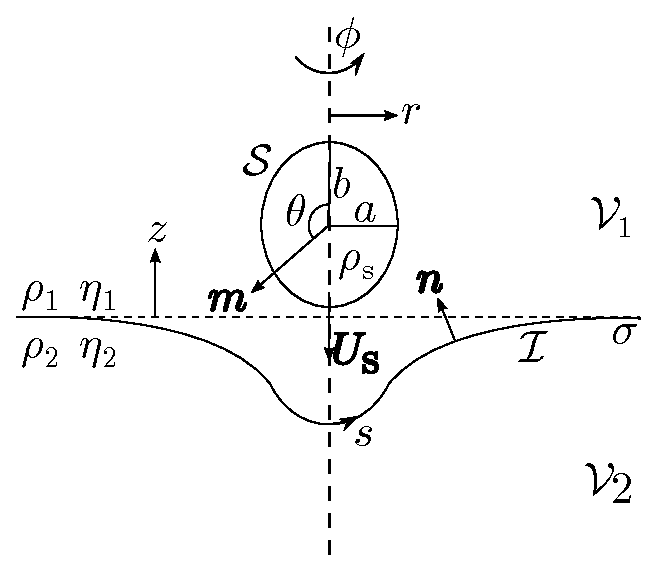
\includegraphics[width=0.8\textwidth]{../../Programming/sinking_bim_write_up/trunk/formulation.eps}$$
    \caption{Diagrammatic representation of the system. A spheroid falls on-axis under gravity, at low Reynolds number, towards an initially horizontal interface between two density stratified, immiscible, semi-infinite fluids. \label{fig:params}}
  \end{figure}


The dimensionless stress tensor for each fluid can be written as

\begin{equation}
\label{equ:nd_stress_def}
T_{l, ij}'(\boldsymbol{x'}) = -P_{\text{d},l}'(\boldsymbol{x'}) \delta_{ij} + \Lambda_{l}[\partial_{i}' u_{l, j}'(\boldsymbol{x'}) - \partial_{j}' u_{l, i}'(\boldsymbol{x'})],
\end{equation}

where $P'_{\text{d},l}$ and $u'_{l,i}$ are the dimensionless dynamic pressure and velcoity fields in fluid $l$ respectively. The parameter $l$ is used to denote the fluid and $i,j$ to denote tensoral components. The parameter $\Lambda_{l}$ is defined as

\begin{equation}
\label{equ:Llambda}
\Lambda_{l} = \frac{\eta_{l}}{\eta_{1}} = \left\{
    \begin{array}{l l}
      1, & \quad \text{for } l = 1 \\
      \frac{\eta_{2}}{\eta_{1}} = \lambda, & \quad \text{for } l = 2,
    \end{array} \right.\ 
\end{equation}

where $\eta_{2}$ is the dynamic viscosity of the lower phase. Note $\lambda$ is the viscosity ratio of the two fluids. Additionally $\mathcal{V}_{1(2)}$ dentotes the volume of fluid 1(2), $\mathcal{I}$ the interface and $\mathcal{S}$ the spheroid surface. $\boldsymbol{m}$ and $\boldsymbol{n}$ are the normal vectors to the spheroid surface and interface respectively and both are directed into fluid 1. Cylindrical polar coordinates are used to describe the system with $r$ the radial coordinate with respect to the symmetry axis, $\phi$ the azimuthal coordinate, and $z$ the vertical coordinate with respect to the plane of the initial, undeformed interface. Additionally, the polar angle $\theta$ is defined with respect to the centre of the spheroid, and the arc-length $s$ is defined as the distance along the interface from the symmetry axis in any azimuthal plane.

It is straightforward to apply the general equations of motion and boundary conditions to the problem (sections~\ref{subsec:EoM} and~\ref{subsec:BC}). The equations of motion, which must be satsified in both fluid domains, appear as 

\begin{equation}
\label{equ:cont}
\partial_{\text{i}}' u_{l,i}'(\boldsymbol{x'}) = 0,
\end{equation}

and 

\begin{equation}
\label{equ:prob_stokes}
\partial_{\text{i}}' T_{l,ij}'(\boldsymbol{x'}) = 0.
\end{equation}

The first boundary condition imposed is that the undisturbed fluid is quiescent, so the velocity field is constrained to decay away from the sphere,

\begin{equation}
\label{equ:BC_inf}
u_{l, i}'(\boldsymbol{x'}) \to 0 \text{ as } |\boldsymbol{x'}| \to \infty.
\end{equation}

The kinematic boundary condition on the fluid interface (equation~\ref{equ:fluid_fluid_kin}) can be expressed as  

\begin{equation}
\label{equ:BC_kin_int_nodim}
u_{1,i}'(\boldsymbol{x'}) = u_{2,i}'(\boldsymbol{x'}), \quad \boldsymbol{x'} \in \mathcal{I}.
\end{equation}

The dynamic boundary condition is also imposed at the interface;

\begin{equation}
\label{equ:BC_dyn_int}
n_{i}(\boldsymbol{x'}) [T_{1, ij}'(\boldsymbol{x'}) - T_{2,ij}'(\boldsymbol{x'})] \Ca + x_{z}' n_{j}(\boldsymbol{x'}) \Bo = n_{j}(\boldsymbol{x'}) \partial_{i}' n_{i}(\boldsymbol{x'}), \quad \text{for } \boldsymbol{x'} \in \mathcal{I}.
\end{equation}

However, the modified density ratio (MDR) D can be defined as

\begin{equation}
\label{equ:dim_dens_rat}
D = \frac{9 \Ca}{2 \Bo} = \frac{\rho_{\text{s}} - \rho_{1}}{\rho_{2} - \rho_{1}}.
\end{equation}

This means equation~\ref{equ:BC_dyn_int} can be re-expressed as

\begin{equation}
\label{equ:d_int}
\frac{9 n_{i}(\boldsymbol{x'}) [T_{1, ij}'(\boldsymbol{x'}) - T_{2, ij}'(\boldsymbol{x'})] D \Bo}{2} = n_{j}(\boldsymbol{x'})[\partial_{i}' n_{i}(\boldsymbol{x'}) - \hat{z}_{i} x_{i}' \Bo] , \quad \text{for } \boldsymbol{x'} \in \mathcal{I}.
\end{equation}

The kinematic boundary condition on the spheroid surface is 

\begin{equation}
\label{equ:BC_kin_spere}
u_{1,i}'(\boldsymbol{x'}) = U_{\text{s},i}', \quad \text{for } \boldsymbol{x'} \in \mathcal{S},
\end{equation}

where $U'_{\text{s},i}$ is the dimensionless velocity of the spheroid. The final boundary condition is the dynamic boundary condition on the spheroid. The force on the fluid due to the spheroid originates from the balance between gravity and buoyancy,

\begin{equation}
\label{equ:sphere_force}
F_{i} = -\frac{4 \pi a^{2} b (\rho_{\text{s}} - \rho_{1}) g \hat{z}_{i}}{3},
\end{equation}

where b is the vertical semi-axis of the spheroid and $\hat{z}_{i}$ is the vertical unit vector. Substituting this into equation~\ref{equ:nodim_fluid_solid} and using equation~\ref{equ:char_vel} results in

\begin{equation}
\label{equ:BC_dyn_sphere}
\int_{\mathcal{S}} f_{i}(\boldsymbol{x'}) \mathrm{d} \mathcal{S}' = -6 \pi \hat{z}_{i}.
\end{equation}

Defining the aspect ratio of the spheroid $R = b / a$, the dimensionless numbers that describe the system are the set $\{\lambda, D, \Bo, R\}$.

\subsection{Integral Representation}
\label{subsec:prob_int_rep}

To recast the problem in an integral representation, equation~\ref{equ:Stokes_int_domain} needs to be applied to each fluid separately. The domain of fluid 1 is bound by the spheroid surface and interface, and extends to infinity as $r, z \to \infty$. The boundary condition at infinity (equation~\ref{equ:BC_inf}) ensures that the far-field contribution to the surface integrals in equation~\ref{equ:Stokes_int_domain} vanishes, meaning that just the spheroid surface and interface contribute. Additionally the no-slip boundary condition on the spheroid surface (equation~\ref{equ:BC_kin_spere}), the divergence theorem (appendix~\ref{app:div_theory}) and the definition of the Greens function for stress (equation~\ref{equ:stress_green_def}) can be used to show that the integral of $u'_{1,i}(\boldsymbol{y'}) K_{ijk}(\boldsymbol{\xi}) m_{j}(\boldsymbol{y'})$ over the spheroid surface vanishes. Hence the boundary integral equation for fluid 1 can be written as 


\begin{align}
\label{equ:bie_fluid1}
\dashint_{\mathcal{S}} J_{ik}(\boldsymbol{\xi}) T'_{1,ij}(\boldsymbol{y'}) m_{j}(\boldsymbol{y'}) \mathrm{d}^{2} \boldsymbol{y'} + \dashint_{\mathcal{I}} J_{ik}(\boldsymbol{\xi}) T'_{1,ij}(\boldsymbol{y'}) n_{j}(\boldsymbol{y'}) \mathrm{d}^{2}\boldsymbol{y'} + \nonumber \\
\dashint_{\mathcal{I}} u'_{1,i}(\boldsymbol{y'}) K_{ijk}(\boldsymbol{\xi}) n_{j}(\boldsymbol{y}) \mathrm{d}^{2}\boldsymbol{y'} = 
\left\{
    \begin{array}{l l}
      \frac{u'_{1,k}(\boldsymbol{x'})}{2} &\quad \text{for } \boldsymbol{x'} \in \mathcal{I}, \\
      u'_{s,k} &\quad \text{for } \boldsymbol{x'} \in \mathcal{S}.
\end{array}
\right.\ 
\end{align}

For fluid 2, the contribution to the surface integrals at infinity again vanishes leaving just a contribution from the interface. Using the kinemtic boundary condition at the interface (equation~\ref{equ:BC_kin_int_nodim}), the boundary integral equation for fluid 2 can be written as

\begin{equation}
\label{equ:bie_fluid2}
-\dashint_{\mathcal{I}} J_{ik}(\boldsymbol{\xi}) T'_{1,ij}(\boldsymbol{y'}) n_{j}(\boldsymbol{y'}) \mathrm{d}^{2}\boldsymbol{y'} - \lambda \dashint_{\mathcal{I}} u'_{1,i}(\boldsymbol{y'}) K_{ijk}(\boldsymbol{\xi}) n_{j}(\boldsymbol{y}) \mathrm{d}^{2}\boldsymbol{y'} = \frac{\lambda u'_{1,k}(\boldsymbol{x'})}{2} \quad \text{for } \boldsymbol{x'} \in \mathcal{I} ,
\end{equation}

where the minus sign occurs since the normal vector is directed out of fluid 2. Equations~\ref{equ:bie_fluid1} and~\ref{equ:bie_fluid2} can be added together and combined with equation~\ref{equ:d_int} to obtain

\begin{align}
\label{equ:I1}
\dashint_{\mathcal{S}} J_{ik}(\boldsymbol{\xi}) f_{\text{s},i}(\boldsymbol{y'}) \mathrm{d}^{2} \boldsymbol{y'} + \frac{9}{2 D \Bo} \dashint_{\mathcal{I}} J_{ik}(\boldsymbol{\xi}) n_{i}(\boldsymbol{y'}) [\partial'_{j} n_{j}(\boldsymbol{y'}) - y'_{z} \Bo] \mathrm{d}^{2} \boldsymbol{y'} + \nonumber \\
(1 - \lambda) \dashint_{\mathcal{I}} u'_{1,i}(\boldsymbol{y'}) K_{ijk}(\boldsymbol{\xi}) n_{j}(\boldsymbol{y'}) \mathrm{d}^{2}\boldsymbol{y'} = 
\left\{
    \begin{array}{l l}
      \frac{(1 + \lambda) u'_{1,k}(\boldsymbol{x'})}{2}, &\quad \text{for } \boldsymbol{x'} \in \mathcal{I}, \\
      u'_{s,k}, &\quad \text{for } \boldsymbol{x'} \in \mathcal{S}.
\end{array}
\right.\ 
\end{align}

This together with equation~\ref{equ:BC_dyn_sphere} completely describes the system in an integral representation. 

\subsection{Axisymmetric Simplification}
\label{subsec:axi_sym}

Exploiting the axial symmetry of the system, to chose the point $\boldsymbol{x'}$ can be chosen such that it lies in the plane defined by $\phi = 0$. Hence in Cartesian coordinates $\boldsymbol{x'} = (x_{r}, 0, x_{z})$. This also means one can write $\boldsymbol{y'} = (y_{r} \cos \phi, y_{r} \sin \phi, y_{z})$. On the surface of the spheroid $y_{r} = y_{r}(\theta)$ and $y_{z} = y_{z}(\theta)$, and on the interface $y_{r} = y_{r}(s)$ and $y_{z} = y_{z}(s)$. Additionally $\boldsymbol{f}_{} = [f_{r}(\theta) \cos \phi, f_{r}(\theta) \sin \phi, f_{z}(\theta)]$ and $\boldsymbol{n} = [n_{r}(s) \cos\phi, n_{r}(s) \sin\phi, n_{z}(s)]$. Since the system is axisymmetric, it is useful to extract the azimuthal integration from the surface integrals in equations~\ref{equ:BC_dyn_sphere} and~\ref{equ:I1}. To achieve this, the Cartesian components of each equation are considered separately. For equation~\ref{equ:I1}, it can be shown that both the left and right hand sides of the 2-component equation are identically zero. To show this, $J_{ij}$ and $K_{ijk}$ are first expanded in terms of in terms of the components of $\boldsymbol{x'}$ and $\boldsymbol{y'}$, before the integration over $\phi$ is carried out. For equation~\ref{equ:BC_dyn_sphere} it can be shown that the 1- and 2-components are identically zero. This leaves three integral equations which can be expressed as

\begin{align}
\label{equ:cont_ie_1}
R \int_{\theta = 0}^{\pi} B_{\alpha\beta}(\boldsymbol{x'},\theta) \Phi_{\beta}(\theta) \mathrm{d}\theta + \int_{s = 0}^{\infty} \left(A_{\alpha\beta}(\boldsymbol{x'},s) y_{r}(s) - \frac{(1 + \lambda)\delta_{\alpha\beta} \delta(s - s_{0})}{2}\right) \Psi_{\beta}(s) \mathrm{d}s \nonumber \\
= - \int_{s = 0}^{\infty} C_{\alpha}(\boldsymbol{x'},s) y_{r}(s) \mathrm{d}s, \quad \text{for } \boldsymbol{x'} \in \mathcal{I},
\end{align}

\begin{align}
\label{equ:cont_ie_2}
R \int_{\theta = 0}^{\pi} B_{\alpha\beta}(\boldsymbol{x'},\theta) \Phi_{\beta}(\theta) \mathrm{d}\theta + \int_{s = 0}^{\infty} A_{\alpha\beta}(\boldsymbol{x'},s) \Psi_{\beta}(s) y_{r}(s) \mathrm{d}s - \Theta_{\alpha} \nonumber \\
= \int_{s = 0}^{\infty} C_{\alpha}(\boldsymbol{x'},s) y_{r}(s) \mathrm{d}s, \quad \text{for } \boldsymbol{x'} \in \mathcal{S}, 
\end{align}

and 

\begin{equation}
\label{equ:cont_ie_3}
\int_{\theta = 0}^{\pi} \Phi_{2}(\theta) \mathrm{d}\theta = -3, 
\end{equation}

where the quantities $\boldsymbol{A}$, $\boldsymbol{B}$, $\boldsymbol{C}$, $\boldsymbol{\Psi}$, $\boldsymbol{\Phi}$ and $\boldsymbol{\Theta}$ are defined as:

\begin{equation}
\setlength{\arraycolsep}{5pt}
\renewcommand{\arraystretch}{1.3}
\boldsymbol{A} = (1 - \lambda) \bigint_{\phi = 0}^{2 \pi} \left( \begin{matrix}
   n_{r}(K_{111} \cos^{2}\phi + K_{221} \sin^{2}\phi &  n_{r}(K_{131} \cos\phi + K_{231} \sin\phi)   \\[-15pt]
{}+ 2 K_{121} \sin\phi \cos\phi) & {}+n_{z}K_{331} \\[-15pt]
{}+n_{z}(K_{131} \cos\phi + K_{231} \sin\phi) & {} \\[-5pt]
   n_{r}(K_{113} \cos^{2}\phi + K_{223} \sin^{2}\phi &   n_{r}(K_{133} \cos\phi + K_{233} \sin\phi)  \\[-15pt]
{}+ 2 K_{123} \sin\phi \cos\phi) & {}+n_{z}K_{333} \\[-15pt]
{}+n_{z}(K_{133} \cos\phi + K_{233} \sin\phi) & {} \\
\end{matrix} \right) \mathrm{d}\phi ,
\label{equ:mat_A}
\end{equation}


\begin{equation}
\setlength{\arraycolsep}{5pt}
\renewcommand{\arraystretch}{1.3}
\boldsymbol{B} = \bigintss_{\phi = 0}^{2 \pi} \left( \begin{matrix}
J_{11} \cos\phi + J_{21} \sin\phi & J_{31} \\[-5pt]
J_{13} \cos\phi + J_{23} \sin\phi & J_{33} \\
\end{matrix} \right) \mathrm{d}\phi ,
\label{equ:mat_B}
\end{equation}


\begin{equation}
\setlength{\arraycolsep}{5pt}
\renewcommand{\arraystretch}{1.3}
\boldsymbol{C} = \frac{9(\partial'_{j} n_{j} - \Bo y_{z})}{2 D \Bo} \bigintss_{\phi = 0}^{2 \pi} \left( \begin{matrix}
n_{r} (J_{11} \cos\phi + J_{21} \sin\phi) + n_{z} J_{31} \\[-5pt]
n_{r} (J_{13} \cos\phi + J_{23} \sin\phi) + n_{z} J_{23} \\
\end{matrix} \right) \mathrm{d}\phi ,
\label{equ:mat_C}
\end{equation}


\begin{equation}
\setlength{\arraycolsep}{5pt}
\renewcommand{\arraystretch}{1.3}
\boldsymbol{\Psi} = \left( \begin{matrix}
u'_{1,r}(s) \\[-5pt]
u'_{1,z}(s) \\
\end{matrix} \right),
\label{equ:vec_a}
\end{equation}


\begin{equation}
\setlength{\arraycolsep}{5pt}
\renewcommand{\arraystretch}{1.3}
\boldsymbol{\Phi} = \left( \begin{matrix}
f_{\text{s},r}(\theta) \\[-5pt]
f_{\text{s},z}(\theta) \\
\end{matrix} \right) \sin^{2}\theta \left(1 + \frac{\cot^{2}\theta}{R^{2}}\right)^{1/2}  ,
\label{equ:vec_b}
\end{equation}

and 

\begin{equation}
\setlength{\arraycolsep}{5pt}
\renewcommand{\arraystretch}{1.3}
\boldsymbol{\Theta} = \left( \begin{matrix}
0 \\[-5pt]
u'_{\text{s}} \\
\end{matrix} \right) .
\label{equ:vec_d}
\end{equation}

For brevity, the function arguments have been dropped from the kernels and the normal vectors but $n_{i} = n_{i}[\boldsymbol{y'}(s, \phi)]$ and in equation~\ref{equ:mat_A}, $K_{ijk} = K_{ijk}[\boldsymbol{x'} - \boldsymbol{y'}(s, \phi)]$, in equation~\ref{equ:mat_B}, $J_{ij} = J_{ij}[\boldsymbol{x'} - \boldsymbol{y'}(\theta, \phi)]$ and in equation~\ref{equ:mat_C}, $J_{ij} = J_{ij}[\boldsymbol{x'} - \boldsymbol{y'}(s, \phi)]$.

The aziumthal integrals inside the definitions of $\boldsymbol{A}$, $\boldsymbol{B}$ and $\boldsymbol{C}$ can be expressed as sums of complete elliptic integrals of the first and second kind \citep{Lee82, Geller86, Graziani89, Pozrikidis92, Manga94, Roumeliotis00} which can then be evaluated using polynomial expansions \citep{Abramowitz72}. Details of this are given in appendices~\ref{app:ellip} and~\ref{app:mat_A}.

\section{Numerical Method}
\label{sec:num_meth}

Equations~\ref{equ:cont_ie_1} to~\ref{equ:cont_ie_3} are a coupled set of integral equations for the unknowns $\boldsymbol{\Psi}(s)$, $\boldsymbol{\Phi}(\theta)$ and $\boldsymbol{\Theta}$. These solutions can be found numerically by discretising the system, allowing the integral equations to be expressed as a linear system of algerbraic equations which are then solved using LU decomposition and Gaussian elimination \citep{Riley06, Press07}. Once the interfacial and sphere velocities are solved for, the system is iterated forward in time, and the process is repeated. 

\subsection{Discretisation and Linear System}
\label{subsec:discrete}

To discretise the set of equations, the interface and spheroid surface are divided into intervals. The interface is divided into $N$ axisymmetric rings, where the $i^{\text{th}}$ ring is centred at arc-length $s_{i}$ and is of thinkness $\Delta_{s,i}$.  The interface is truncated at the arc-length $s_{N}$. The sphere surface is discretised in $M$ axisymmetric rings, where the $i^{\text{th}}$ ring is centred at polar coordinate $\theta_{i}$ and has a thickness $\Delta_{\theta,i}$. A schematic of the discretisation scheme is depicted in figure~\ref{fig:discrete}. 

  \begin{figure}
    $$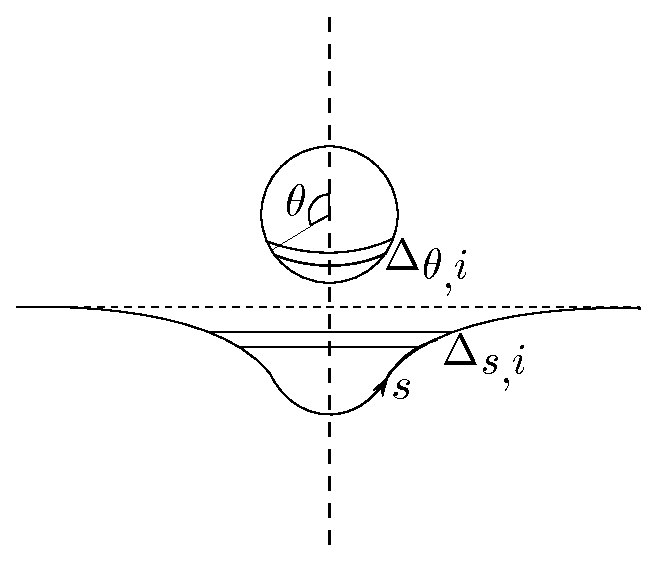
\includegraphics[width=0.8\textwidth]{../../Programming/sinking_bim_write_up/trunk/discrete.eps}$$
    \caption{Diagrammatic representation of the discretisation of the system. Both interface and spheroid surface are divided into axisymmetric rings centred on the symmetry axis. \label{fig:discrete}}
  \end{figure}

One then chooses $\boldsymbol{x'} = \boldsymbol{x}_{i}$ where $\boldsymbol{x}_{i} = \boldsymbol{x}_{i}(\theta_{i})$ on $\mathcal{S}$ and $\boldsymbol{x}_{i} = \boldsymbol{x}_{i}(s_{i})$ on $\mathcal{I}$. That is, the point $\boldsymbol{x'}$ is chosen to be the midpoint of one of the intervals. The integrals in equations~\ref{equ:cont_ie_1} to~\ref{equ:cont_ie_3} can then be expressed as discrete sums of integrals over each element. The approximation is then made that the unknowns $\boldsymbol{\Psi}(s)$ and $\boldsymbol{\Phi}(\theta)$ are constant over the width of an interval such that for interval $i$, $\boldsymbol{\Psi}(s) = \boldsymbol{\Psi}(s_{i})$ and $\boldsymbol{\Phi}(\theta) = \boldsymbol{\Phi}(\theta_{i})$. This gives the discrete form of the integral equations:

\begin{align}
\label{equ:dis_ie_1}
R \sum_{i = 1}^{M} \Phi_{\beta}(\theta_{i}) \int_{\Delta_{\theta,i}} B_{\alpha\beta}(s_{j},\theta) \mathrm{d}\theta + \sum_{i=1}^{N} \Psi_{\beta}(s_{i}) \int_{\Delta_{s,i}} \left(A_{\alpha\beta}(s_{j},s) y_{r}(s) - \frac{(1 + \lambda) \delta_{\alpha\beta} \delta(s - s_{j})}{2}\right) \mathrm{d}s \nonumber \\
= - \sum_{i = 1}^{N} \int_{\Delta_{s,i}} C_{\alpha}(s_{j},s) y_{r}(s) \mathrm{d}s,
\end{align}

\begin{align}
\label{equ:dis_ie_2}
R \sum_{i = 1}^{M} \Phi_{\beta}(\theta_{i}) \int_{\Delta_{\theta,i}} B_{\alpha\beta}(\theta_{j},\theta) \mathrm{d}\theta + \sum_{i=1}^{N} \Psi_{\beta}(s_{i}) \int_{\Delta_{s,i}} A_{\alpha\beta}(\theta_{j},s) y_{r}(s) \mathrm{d}s - \Theta_{\alpha} \nonumber \\
= - \sum_{i = 1}^{N} \int_{\Delta_{s,i}} C_{\alpha}(\theta_{j},s) y_{r}(s) \mathrm{d}s,
\end{align}

and 

\begin{equation}
\label{equ:dis_ie_3}
\sum_{i = 1}^{M} \Phi_{2}(\theta_{i}) \int_{\Delta_{\theta,i}} \mathrm{d}\theta = -3.
\end{equation}

This is seemingly a set of $2(N + M) + 1$ linear equations for $2(N + M) + 1$ unknowns: $\Phi_{\alpha}(\theta_{i})$, $\Psi_{\alpha}(s_{j})$ and $\Theta_{1}$ (recall that $\Theta_{2} = 0$), where $\alpha = 1,2$, $i = 1,2,...,M$ and $j = 1,2,...,N$. However, physical arguments can be used to simplify the system further. First, by symmetry, the radial interfacial velocity must vanish on the symmetry axis i.e. $\Psi_{1}(s_{1}) = 0$. Additionally, the on-axis radial tractions on the sphere must also vanish meaning $\Phi_{1}(\theta_{1}) = \Phi_{1}(\theta_{M}) = 0$. Indeed, by using the expressions for $A_{\alpha\beta}$, $B_{\alpha\beta}$ and $C_{\alpha}$ given in appendix~\ref{subapp:spec_case}, it can be shown that the coefficients of these terms vanish. Hence the equations where these terms appear are redundant and can be removed from the linear system. This leaves a system of $2(N + M - 1)$ linear equations for $2(N + M - 1)$ unknowns.

\subsection{Evaluation of the coefficients}
\label{subsec:eval_coeff}

These equations can be recast as a matrix equation $L_{\mu\nu} X_{\mu} = Y_{\nu}$ where the unknown quantities are the elements $X_{\mu}$. The elements $L_{\mu\nu}$ and $Y_{\nu}$ are the coefficients of the system and contain integrals that need to be evaluated numerically. If $\boldsymbol{x'}_{j}$ is not within the range of integration, then this is done using 4-point Gaussian-Legendre quadrature \citep{Riley06}. However if $\boldsymbol{x'}_{j}$ is in the integration range, then the integrand might be singular at the point $\boldsymbol{y'} = \boldsymbol{x'}_{j}$, and care needs to be taken when evaluating the integral. First, the order of the singularity needs to be determined. To do this, write $\boldsymbol{y'} = \boldsymbol{x'}_{j} + \epsilon \boldsymbol{t}$, where $\epsilon = \theta - \theta_{j}$ on the sphere or $\epsilon = s - s_{j}$ on the interface, and $\boldsymbol{t}$ is the tangent to the curve at the point $\boldsymbol{x'}$. The integrands are then expanded in terms of $\epsilon$. The first singular term is the leading order contribution to the integrand, and the order of the singularity is the order of this term. Table~\ref{tab:sing} shows the order of the singularity of each component of $\boldsymbol{A}$, $\boldsymbol{B}$ and $\boldsymbol{C}$.

\begin{table}
\centering
\caption{The order of the singularity of the components of $\boldsymbol{A}$, $\boldsymbol{B}$ and $\boldsymbol{C}$. \label{tab:sing}}
\begin{tabular}{|c|c||c|c||c|c|}
  \hline
  $A_{11}$ & $1 / \epsilon$ & $B_{11}$ & $\ln|\epsilon|$ & $C_{1}$  & $\ln|\epsilon|$\\
  $A_{12}$ & 0 & $B_{12}$ & 0 & $C_{2}$  & $\ln|\epsilon|$\\
  $A_{21}$ & 0 & $B_{21}$ & 0  &   & \\
  $A_{22}$ & 0 & $B_{22}$ & $\ln|\epsilon|$ &   & \\
  \hline
\end{tabular} 
\end{table}

The integrand is then re-written as the sum of a regular and singular part. Denoting the integrand by $I(\zeta, \zeta_{i})$ (where $\zeta$ represents $\theta$ or $s$ depending on whether the integration is over the sphere or the interface), this can be written as $I(\zeta, \zeta_{i}) = I_{r}(\zeta, \zeta_{i}) + I_{s}(\zeta, \zeta_{i})$ where $I_{r}$ is the regular part and $I_{s}$ is the singular part. The singular part can then be written as

\begin{equation}
\label{equ:sing_meth}
I(\zeta, \zeta_{i})_{s} = [I_{s}(\zeta, \zeta_{i}) -L(\zeta, \zeta_{i})] + L(\zeta, \zeta_{i}),
\end{equation}

where $L$ is the leading order contribution to $I_{s}$. The terms in square parenthesese now form a regular function which can be integrated numerically. For the case that the integral is $1/\epsilon$ singular, the final term can be expressed as

\begin{equation}
\label{equ:recip_sing}
L(\zeta, \zeta_{i}) = \frac{g(\zeta, \zeta_{i})}{\epsilon} = \frac{g(\zeta, \zeta_{i}) - g(\zeta_{i}, \zeta_{i})}{\epsilon} + \frac{g(\zeta_{i}, \zeta_{i})}{\epsilon},
\end{equation}

where $g(\zeta, \zeta_{i})$ is a regular function. Similarly, if the integral if $\ln|\epsilon|$ singular

\begin{equation}
\label{equ:ln_sing}
L(\zeta, \zeta_{i}) = g(\zeta, \zeta_{i}) \ln|\epsilon| = [g(\zeta, \zeta_{i}) - g(\zeta_{i}, \zeta_{i})]\ln|\epsilon| + g(\zeta_{i}, \zeta_{i})\ln|\epsilon|
\end{equation}

In both these cases, the first term on the right hand side is regular (since it vanishes when $\zeta = \zeta_{i}$) and the last term is singular but can be integrated analytically. This means that the irregular integrand can be expressed as the sum of a regular function, that can be integrated numerically, and an irregular function, that can be integrated analytically. 
 
To evaluate integrands on the interface, it is necessary to evaluate the components of the normal vector and its divergence at discrete points along the interface. To do this, the interface is described parametrically with $r = r(s)$ and $z = z(s)$ where cubic splines are fitted to the collocation points describing the interface (WAITING FOR DE BOER BOOK TO REF THIS) using routines given in \citet{Press07}. Remembering that for a surface $H(r,z) = z - f(r)$, the components of the normal vector are given by $n_{i} = \partial_{i} H / (\partial_{j}H \partial_{j}H)$ \citep{Riley06}, the following expressions can be obtained

\begin{equation}
\label{equ:norm_rad}
n_{r}(s) = \frac{-\dot{z}}{(\dot{r} + \dot{z})^{1/2}},
\end{equation}

\begin{equation}
\label{equ:norm_vert}
n_{z}(s) = \frac{\dot{r}}{(\dot{r} + \dot{z})^{1/2}},
\end{equation}

and 

\begin{equation}
\label{equ:div_norm}
\partial'_{i} n_{i} = \frac{\dot{z}}{r (\dot{r} + \dot{z})^{1/2}} + \frac{\dot{r} \ddot{z} - \ddot{r} \dot{z}}{(\dot{r} + \dot{z})^{3/2}}.
\end{equation}

These expressions are given in given in \citep{Manga94} except for a minus sign error in the components of the normal. The derivatives of the splines are calculated numerically using routines modified from \citet{Press07}. 

Once all of the elements $L_{\mu\nu}$ and $Y_{\nu}$ have been calculated the system of equations is solved by Lower-Upper (LU) decomposition and Gaussian elimination \citep{Riley06, Press07} using routines from the GNU Scientific Library (GSL) \citep{Galassi09}.

\subsection{Temporal Iteration}
\label{subsec:time}

The system is iterated forward in time using an explicit first order Euler method \citep{Manga94} with timestep $\Delta t$. This means the position of the sphere $z_{s}$ at time $t + \Delta t$ is found using

\begin{equation}
\label{equ:sphere_it}
z_{s}(t' + \Delta t') = U'_{s}(t) \Delta t',
\end{equation}

and the position of the collocation points on the interface moves according to

\begin{equation}
\label{equ:int_it}
x_{r}(s_{i}, t' + \Delta t') = u_{r}(s_{i},t') \Delta t',
\end{equation}

and

\begin{equation}
\label{equ:int_it}
x_{z}(s_{i}, t' + \Delta t') = u_{z}(s_{i},t') \Delta t'.
\end{equation}

There are both numerical and physical constraints on the value of the timestep. Numerically, it is limited by the Courant-Friedrich-Lewy (CFL) criterion \citep{Courant28}. Physically, it is neccessary to ensure that it is smaller than the timescale over which different processes can occur. Owing to the multi-component nature of this problem, there are four timescales instrinsic to the problem: the Stokes timescale in the upper fluid $\tau_{\text{s},1} = 9 \eta_{1} / [2 (\rho_{\text{s}} - \rho_{1}) g a]$, the Stokes timescale in the lower fluid $\tau_{\text{s},2} = 9 \eta_{2} / [2 (\rho_{\text{s}} - \rho_{2}) g a]$, the capilary time for the upper fluid $\tau_{\text{c},1} = \eta_{1} a / \sigma$ and the capilary time for the lower fluid $\tau_{\text{c},2} = \eta_{2} a / \sigma$. It is required that the timestep is smaller than all of these, so that the physics occuring on each timescale can be resolved. Non-dimensionalising each of these timescales we find that in dimensionless form they exist as $\tau'_{\text{s},1} = 1$, $\tau'_{\text{s},2} = \lambda D / (D - 1)$, $\tau'_{\text{c},1} = 2 D \Bo / 9$, $\tau'_{\text{c},2} = 2 D \Bo \lambda / 9$. Hence, for each simulation, the shortest physical timescale is identified and the timestep is constrained to be smaller than this throughout the simulation. The timestep is allowed to change during the simulation such that it is as large as can be allowed by both the CFL and numerical criteria.


Due to gradients in the velocity tangential to the fluid interface, the distribution of collocation points is altered during this time stepping process, so the collocation points are redistributed between each time step. The collocation points are always uniformly distributed with respect to $s$ on the interface and $\theta$ on the spheroid. Following the redistribution, the linear system is reconstructed for the new geometry and solved using the same procedure. The iteration continues in this fashion until a pre-defined termination criteria is satisfied.

\subsection{Model Termination}
\label{subsec:term}

The model terminates when one of three termination criteria are satisfied:

\begin{enumerate}
\item Separation between spheroid and interface becomes comparable to local separation between collocation points \\
\item Separation between two non-local points of the interface becomes comparable to local separation between collocation points \\
\item A pre-defined maximum number of time steps has been reached \\
\end{enumerate}

The first two criteria are imposed because once the separation between surfaces becomes comparable to the scale at which the surfaces are being discretised the discrete approximation to the continuous system no longer becomes valid. The third criteria is purely defined to prevent the model running indefinitely and if this is satisfied, it can suggest 1) velocities in the system have become so small that the system has effectively reached static equilibrium, or 2) the velocities are only small relative to the time-step and the system is still evolving. It is necessary to examine the model results to determine which of these is the case.

The second termination criteria provides a means to evaluate both the volume of upper phase fluid entrained by the passage of the sphere and the sinking timescale. This is because this criteria is satisfied when the tail of upper phase fluid behind the sphere becomes too thin to be accurately modelled. The assumption is made that the tail snaps at this point in space and time, leading to both the sphere and a finite volume of upper phase fluid losing contact with the bulk of the upper phase. This volume of fluid $V$ is defined as the entrained volume and the sinking timescale $t_{\text{s}}$ is defined as the time between the moment the spheroid first touches the plane of the undeformed interface ($z' = 0$) and the moment at which the tail snaps (when the model terminates). These quantities can only be avaluated for simulations where the tail thickness termination criteria is fullfilled and the next section addresses the regions of the parameter space for which this is observed. 

\section{Model Testing}
\label{sec:test}

This section describes the testing of the numerical model. A common method of testing models is by reproducing a known solution of a related problem. To this end, the numerical method described above has been applied to the problem of the on-axis gravitational settling of a spheroid through a uniform fluid of infinite extend (section~\ref{subsec:no_interf}). Additionally, the numerical model has a number of auxillery parameters: the initial height of the spheroid, the truncation radius of the interface, the number of collocation points on both the sphere and the interface and the step size used in the numerical differentiation of the splines $r = r(s)$ and $z = z(s)$ that describe the interface. Values of these parameters need to be chosen such that the model results are independent of these and this section describes how these values have been obtained. Additionally, model outputs have been compared against experimental observations to provide validation for the model results, and determine how the model performs in different regions of the parameter space.

\subsection{Uniform and Infinite Fluid}
\label{subsec:no_interf}

To test the model, we can remove the interface and fluid 2, leaving us with the problem of the steady gravitational settling of a spheroid through fluid 1, which is uniform and infinite in extent. The terminal velocity of a spheroid settling on axis can be solved for analytically \citep{Happel73} and in our dimensionless scheme is given by

\begin{equation}
\label{equ:term_vel}
U'_{t} = \frac{1}{K},
\end{equation}

where

\begin{equation}
\label{equ:Stokes_corr}
K = \begin{cases}
    \frac{4}{3 (\mu^{2} + 1)^{1/2} [\mu - (\mu^{2} - 1) \cot^{-1} \mu]}       & \quad \text{for } R < 1\\
    \frac{4}{3 (\mu^{2} - 1)^{1/2} [(\mu^{2} + 1) \coth^{-1}\mu - \mu]}  & \quad \text{for } R > 1\\
    1 & \quad \text{for } R = 1, \\
  \end{cases}
\end{equation}

and 

\begin{equation}
\label{equ:Stokes_const}
\mu = \frac{R}{|R^{2} - 1|^{1/2}}.
\end{equation}

For the case that $\lambda = 1$, and a flat interface, the integrals over the interface in equations~\ref{equ:dis_ie_1} to~\ref{equ:dis_ie_3} vanish and the system reduces to that of the case of a spheroid settling in an infinite and uniform fluid. Figure~\ref{fig:Happel_test} shows the analytical result for the terminal velocity from \citet{Happel73} compared with that calculated by our model. It can be seen that agreement is excellent for aspect ratios in the range 0.1-10.

  \begin{figure}
    \input{../../Programming/sinking_bim_write_up/trunk/Happel.tex}
    \caption{Curve shows analytical solution for dimensionless terminal velocity vs. aspect ratio (equation~\ref{equ:Stokes_corr}). Points show calculated values from model. There is excellent agreement for oblate spheroids but the error increases with aspect ratio. \label{fig:Happel_test}}
  \end{figure}

We tested the senstivity of the results to the number of intervals on the sphere. Figure~\ref{fig:int_vel_test} shows the fractional error on the calculated terminal velocity as a function of the number of intervals used to discretise the sphere $M$, for both a prolate and oblate spheroid, and a sphere. For $M \geq 100$, the fractional error is less than 0.003. It is also clear here that the error increases with $R$. 

  \begin{figure}
    \input{../../Programming/sinking_bim_write_up/trunk/int_test.tex}
    \caption{Plot showing the fractional error on the calculated terminal velocity of a spheroid in an infinite and uniform fluid as a function of the number of intervals used to discretise the particle surface. Results are shown for $R = 0.5$, $1$ and $2$. When 100 intervals are used, the fractional error is less than 0.003 and this decreases as the number of intervals increases. It can also be seen that as $R$ increases so does the error. \label{fig:int_vel_test}}
  \end{figure}

\subsection{Initial Height of Sphere}
\label{subsec:init_pos}

The interface will deform as the particle approaches and so we require the initial position of the particle to be far enough above the interface that the results are insensitive to the initial position. We tested the model for parameter values $R = 1$, $D = 10 $, $\Bo = 1000$ and both $\lambda = 0.1$ and $\lambda = 10$. Figure~\ref{fig:height_test_pos} shows the position of the sphere against time for the different viscosity ratios. The time $t = 0$ is defined as the moment when $z_{\text{s}} = 0$. It is seen that the position curves converge for an initial position greater than or equal to 5 sphere radii above the interface. Figure~\ref{fig:height_vol_test} shows that the same is true when considering the volume of upper phase fluid entrained below the plane $z = 0$.

    \begin{figure}
      \centering
      \begin{subfigure}[b]{0.5\textwidth}
        \resizebox{\textwidth}{!}{\Large \input{../../Programming/sinking_bim_write_up/trunk/viscos_rat=0_1_pos_pub.tex}}
        \caption{}
        \label{fig:height_test_pos_tail}
      \end{subfigure}%
      ~
      \begin{subfigure}[b]{0.5\textwidth}
        \resizebox{\textwidth}{!}{\Large \input{../../Programming/sinking_bim_write_up/trunk/viscos_rat=10_pos_pub.tex}}
        \caption{}
        \label{fig:height_test_pos_film}
      \end{subfigure}
      \caption{Plot of the vertical position of a sphere versus time for different initial sphere positions for $D = 10$ and $\Bo = 1000$. a) $\lambda = 0.1$ - For initial positions greater or equal than 5 radii above the interface, the position curves quickly converge. b) $\lambda = 10$ - For initial positions greater or equal than 5 radii above the interface, the position curves are indistingusihable. For an initial position of 3, the curve quickly converges to the others.}\label{fig:height_test_pos}
    \end{figure}

  \begin{figure}
        \input{../../Programming/sinking_bim_write_up/trunk/viscos_rat=0_1_vol_pub.tex}
    \caption{Curves showing the volume of upper phase fluid entrained below the plane $z = 0$ as a function of time, for different initial sphere positions and $D = 10$, $\Bo = 1000$ and $\lambda = 0.1$. It is seen that the curves converge for an initial position greater than or equal to 5 sphere radii above the interface. \label{fig:height_vol_test}}
  \end{figure}

\subsection{Truncation Length}
\label{subsec:trunc_length}

The model is also tested for its sentitivity with respect to the radial coordinate $r = r_{N}$ at which the interface is truncated. Figure~\ref{fig:trunc_test_pos} shows the position of the sphere as a function of time for different $r_{N}$. It is seen that for $r_{N} \geq 10$ there is no change to the results. Figure~\ref{fig:trunc_vol_test} shows the dependence of the entrained volume as a function of time on the truncation radius. For $r_{N} \geq 20$ the curves are identical from the start of the simulation, and for $r_{N} = 10$ the curve converges to the others during the run.


    \begin{figure}
      \centering
      \begin{subfigure}[b]{0.5\textwidth}
        \resizebox{\textwidth}{!}{\Large \input{../../Programming/sinking_bim_write_up/trunk/viscos_rat=0_1_pos_trunc_pub.tex}}
        \caption{}
        \label{fig:trunc_test_pos_tail}
      \end{subfigure}%
      ~
      \begin{subfigure}[b]{0.5\textwidth}
        \resizebox{\textwidth}{!}{\Large % GNUPLOT: LaTeX picture with Postscript
\begingroup
  \makeatletter
  \providecommand\color[2][]{%
    \GenericError{(gnuplot) \space\space\space\@spaces}{%
      Package color not loaded in conjunction with
      terminal option `colourtext'%
    }{See the gnuplot documentation for explanation.%
    }{Either use 'blacktext' in gnuplot or load the package
      color.sty in LaTeX.}%
    \renewcommand\color[2][]{}%
  }%
  \providecommand\includegraphics[2][]{%
    \GenericError{(gnuplot) \space\space\space\@spaces}{%
      Package graphicx or graphics not loaded%
    }{See the gnuplot documentation for explanation.%
    }{The gnuplot epslatex terminal needs graphicx.sty or graphics.sty.}%
    \renewcommand\includegraphics[2][]{}%
  }%
  \providecommand\rotatebox[2]{#2}%
  \@ifundefined{ifGPcolor}{%
    \newif\ifGPcolor
    \GPcolorfalse
  }{}%
  \@ifundefined{ifGPblacktext}{%
    \newif\ifGPblacktext
    \GPblacktexttrue
  }{}%
  % define a \g@addto@macro without @ in the name:
  \let\gplgaddtomacro\g@addto@macro
  % define empty templates for all commands taking text:
  \gdef\gplbacktext{}%
  \gdef\gplfronttext{}%
  \makeatother
  \ifGPblacktext
    % no textcolor at all
    \def\colorrgb#1{}%
    \def\colorgray#1{}%
  \else
    % gray or color?
    \ifGPcolor
      \def\colorrgb#1{\color[rgb]{#1}}%
      \def\colorgray#1{\color[gray]{#1}}%
      \expandafter\def\csname LTw\endcsname{\color{white}}%
      \expandafter\def\csname LTb\endcsname{\color{black}}%
      \expandafter\def\csname LTa\endcsname{\color{black}}%
      \expandafter\def\csname LT0\endcsname{\color[rgb]{1,0,0}}%
      \expandafter\def\csname LT1\endcsname{\color[rgb]{0,1,0}}%
      \expandafter\def\csname LT2\endcsname{\color[rgb]{0,0,1}}%
      \expandafter\def\csname LT3\endcsname{\color[rgb]{1,0,1}}%
      \expandafter\def\csname LT4\endcsname{\color[rgb]{0,1,1}}%
      \expandafter\def\csname LT5\endcsname{\color[rgb]{1,1,0}}%
      \expandafter\def\csname LT6\endcsname{\color[rgb]{0,0,0}}%
      \expandafter\def\csname LT7\endcsname{\color[rgb]{1,0.3,0}}%
      \expandafter\def\csname LT8\endcsname{\color[rgb]{0.5,0.5,0.5}}%
    \else
      % gray
      \def\colorrgb#1{\color{black}}%
      \def\colorgray#1{\color[gray]{#1}}%
      \expandafter\def\csname LTw\endcsname{\color{white}}%
      \expandafter\def\csname LTb\endcsname{\color{black}}%
      \expandafter\def\csname LTa\endcsname{\color{black}}%
      \expandafter\def\csname LT0\endcsname{\color{black}}%
      \expandafter\def\csname LT1\endcsname{\color{black}}%
      \expandafter\def\csname LT2\endcsname{\color{black}}%
      \expandafter\def\csname LT3\endcsname{\color{black}}%
      \expandafter\def\csname LT4\endcsname{\color{black}}%
      \expandafter\def\csname LT5\endcsname{\color{black}}%
      \expandafter\def\csname LT6\endcsname{\color{black}}%
      \expandafter\def\csname LT7\endcsname{\color{black}}%
      \expandafter\def\csname LT8\endcsname{\color{black}}%
    \fi
  \fi
    \setlength{\unitlength}{0.0500bp}%
    \ifx\gptboxheight\undefined%
      \newlength{\gptboxheight}%
      \newlength{\gptboxwidth}%
      \newsavebox{\gptboxtext}%
    \fi%
    \setlength{\fboxrule}{0.5pt}%
    \setlength{\fboxsep}{1pt}%
\begin{picture}(7200.00,5040.00)%
    \gplgaddtomacro\gplbacktext{%
      \csname LTb\endcsname%
      \put(682,704){\makebox(0,0)[r]{\strut{}$-1$}}%
      \put(682,1317){\makebox(0,0)[r]{\strut{}$0$}}%
      \put(682,1929){\makebox(0,0)[r]{\strut{}$1$}}%
      \put(682,2542){\makebox(0,0)[r]{\strut{}$2$}}%
      \put(682,3154){\makebox(0,0)[r]{\strut{}$3$}}%
      \put(682,3767){\makebox(0,0)[r]{\strut{}$4$}}%
      \put(682,4379){\makebox(0,0)[r]{\strut{}$5$}}%
      \put(814,484){\makebox(0,0){\strut{}$-10$}}%
      \put(1563,484){\makebox(0,0){\strut{}$-8$}}%
      \put(2311,484){\makebox(0,0){\strut{}$-6$}}%
      \put(3060,484){\makebox(0,0){\strut{}$-4$}}%
      \put(3809,484){\makebox(0,0){\strut{}$-2$}}%
      \put(4557,484){\makebox(0,0){\strut{}$0$}}%
      \put(5306,484){\makebox(0,0){\strut{}$2$}}%
      \put(6054,484){\makebox(0,0){\strut{}$4$}}%
      \put(6803,484){\makebox(0,0){\strut{}$6$}}%
    }%
    \gplgaddtomacro\gplfronttext{%
      \csname LTb\endcsname%
      \put(176,2541){\rotatebox{-270}{\makebox(0,0){\strut{}$z_{\text{c}}$}}}%
      \put(3808,154){\makebox(0,0){\strut{}$t$}}%
      \put(3808,4709){\makebox(0,0){\strut{}$\lambda = 10$, $D = 10$, $\Bo = 1000$}}%
      \put(5483,4151){\makebox(0,0){\strut{}Truncation Radius   }}%
      \csname LTb\endcsname%
      \put(4823,3931){\makebox(0,0)[r]{\strut{}10}}%
      \csname LTb\endcsname%
      \put(4823,3601){\makebox(0,0)[r]{\strut{}20}}%
      \csname LTb\endcsname%
      \put(4823,3271){\makebox(0,0)[r]{\strut{}30}}%
      \csname LTb\endcsname%
      \put(4823,2941){\makebox(0,0)[r]{\strut{}40}}%
      \csname LTb\endcsname%
      \put(4823,2611){\makebox(0,0)[r]{\strut{}50}}%
    }%
    \gplbacktext
    \put(0,0){\includegraphics{viscos_rat=10_pos_trunc_pub}}%
    \gplfronttext
  \end{picture}%
\endgroup
}
        \caption{}
        \label{fig:trunc_test_pos_film}
      \end{subfigure}
      \caption{Plot of the vertical position of a sphere versus time for different truncation radii for $D = 10$, $\Bo = 1000$ and both $\lambda = 0.1$ (a) and $\lambda = 10$ (b). The curves are identical for all truncation radii greater than or equal to 10.}\label{fig:trunc_test_pos}
    \end{figure}

  \begin{figure}
    \resizebox{\textwidth}{!}{\Large \input{../../Programming/sinking_bim_write_up/trunk/viscos_rat=0_1_vol_trunc_pub.tex}}
    \caption{Curves showing the volume of upper phase fluid entrained below the plane $z = 0$ as a function of time, for different truncation radii and $D = 10$, $\Bo = 1000$ and $\lambda = 0.1$. It is seen that the curves for $r_{N} \geq 20$ are identical from the start of the simulation, although the curve for $r_{N} = 10$ converges to the other curves during the run. \label{fig:trunc_vol_test}}
  \end{figure}

\subsection{Discretisation of Interface}
\label{subsec:interf}

The number of elements used to discretise the fluid interface $N$ needs to be large enough that the model output is independent of $N$. Figure~\ref{fig:n_interf_test_pos} shows the vertical position of the sphere as a function of time for different $N$. It can be seen that for $N \geq 50$ the curves are independent of $N$. However, the larger the value of $N$ the longer the duration of the simulation. This is because larger values of $N$ allow smaller separations between surfaces to be tolerated. 

    \begin{figure}
      \centering
      \begin{subfigure}[b]{0.5\textwidth}
        \resizebox{\textwidth}{!}{\Large \input{../../Programming/sinking_bim_write_up/trunk/viscos_rat=0_1_pos_n_interf.tex}}
        \caption{}
        \label{fig:n_interf_test_pos_tail}
      \end{subfigure}%
      ~
      \begin{subfigure}[b]{0.5\textwidth}
        \resizebox{\textwidth}{!}{\Large % GNUPLOT: LaTeX picture with Postscript
\begingroup
  \makeatletter
  \providecommand\color[2][]{%
    \GenericError{(gnuplot) \space\space\space\@spaces}{%
      Package color not loaded in conjunction with
      terminal option `colourtext'%
    }{See the gnuplot documentation for explanation.%
    }{Either use 'blacktext' in gnuplot or load the package
      color.sty in LaTeX.}%
    \renewcommand\color[2][]{}%
  }%
  \providecommand\includegraphics[2][]{%
    \GenericError{(gnuplot) \space\space\space\@spaces}{%
      Package graphicx or graphics not loaded%
    }{See the gnuplot documentation for explanation.%
    }{The gnuplot epslatex terminal needs graphicx.sty or graphics.sty.}%
    \renewcommand\includegraphics[2][]{}%
  }%
  \providecommand\rotatebox[2]{#2}%
  \@ifundefined{ifGPcolor}{%
    \newif\ifGPcolor
    \GPcolorfalse
  }{}%
  \@ifundefined{ifGPblacktext}{%
    \newif\ifGPblacktext
    \GPblacktexttrue
  }{}%
  % define a \g@addto@macro without @ in the name:
  \let\gplgaddtomacro\g@addto@macro
  % define empty templates for all commands taking text:
  \gdef\gplbacktext{}%
  \gdef\gplfronttext{}%
  \makeatother
  \ifGPblacktext
    % no textcolor at all
    \def\colorrgb#1{}%
    \def\colorgray#1{}%
  \else
    % gray or color?
    \ifGPcolor
      \def\colorrgb#1{\color[rgb]{#1}}%
      \def\colorgray#1{\color[gray]{#1}}%
      \expandafter\def\csname LTw\endcsname{\color{white}}%
      \expandafter\def\csname LTb\endcsname{\color{black}}%
      \expandafter\def\csname LTa\endcsname{\color{black}}%
      \expandafter\def\csname LT0\endcsname{\color[rgb]{1,0,0}}%
      \expandafter\def\csname LT1\endcsname{\color[rgb]{0,1,0}}%
      \expandafter\def\csname LT2\endcsname{\color[rgb]{0,0,1}}%
      \expandafter\def\csname LT3\endcsname{\color[rgb]{1,0,1}}%
      \expandafter\def\csname LT4\endcsname{\color[rgb]{0,1,1}}%
      \expandafter\def\csname LT5\endcsname{\color[rgb]{1,1,0}}%
      \expandafter\def\csname LT6\endcsname{\color[rgb]{0,0,0}}%
      \expandafter\def\csname LT7\endcsname{\color[rgb]{1,0.3,0}}%
      \expandafter\def\csname LT8\endcsname{\color[rgb]{0.5,0.5,0.5}}%
    \else
      % gray
      \def\colorrgb#1{\color{black}}%
      \def\colorgray#1{\color[gray]{#1}}%
      \expandafter\def\csname LTw\endcsname{\color{white}}%
      \expandafter\def\csname LTb\endcsname{\color{black}}%
      \expandafter\def\csname LTa\endcsname{\color{black}}%
      \expandafter\def\csname LT0\endcsname{\color{black}}%
      \expandafter\def\csname LT1\endcsname{\color{black}}%
      \expandafter\def\csname LT2\endcsname{\color{black}}%
      \expandafter\def\csname LT3\endcsname{\color{black}}%
      \expandafter\def\csname LT4\endcsname{\color{black}}%
      \expandafter\def\csname LT5\endcsname{\color{black}}%
      \expandafter\def\csname LT6\endcsname{\color{black}}%
      \expandafter\def\csname LT7\endcsname{\color{black}}%
      \expandafter\def\csname LT8\endcsname{\color{black}}%
    \fi
  \fi
    \setlength{\unitlength}{0.0500bp}%
    \ifx\gptboxheight\undefined%
      \newlength{\gptboxheight}%
      \newlength{\gptboxwidth}%
      \newsavebox{\gptboxtext}%
    \fi%
    \setlength{\fboxrule}{0.5pt}%
    \setlength{\fboxsep}{1pt}%
\begin{picture}(7200.00,5040.00)%
    \gplgaddtomacro\gplbacktext{%
      \csname LTb\endcsname%
      \put(682,704){\makebox(0,0)[r]{\strut{}$-8$}}%
      \put(682,1229){\makebox(0,0)[r]{\strut{}$-6$}}%
      \put(682,1754){\makebox(0,0)[r]{\strut{}$-4$}}%
      \put(682,2279){\makebox(0,0)[r]{\strut{}$-2$}}%
      \put(682,2804){\makebox(0,0)[r]{\strut{}$0$}}%
      \put(682,3329){\makebox(0,0)[r]{\strut{}$2$}}%
      \put(682,3854){\makebox(0,0)[r]{\strut{}$4$}}%
      \put(682,4379){\makebox(0,0)[r]{\strut{}$6$}}%
      \put(814,484){\makebox(0,0){\strut{}$-10$}}%
      \put(1670,484){\makebox(0,0){\strut{}$0$}}%
      \put(2525,484){\makebox(0,0){\strut{}$10$}}%
      \put(3381,484){\makebox(0,0){\strut{}$20$}}%
      \put(4236,484){\makebox(0,0){\strut{}$30$}}%
      \put(5092,484){\makebox(0,0){\strut{}$40$}}%
      \put(5947,484){\makebox(0,0){\strut{}$50$}}%
      \put(6803,484){\makebox(0,0){\strut{}$60$}}%
    }%
    \gplgaddtomacro\gplfronttext{%
      \csname LTb\endcsname%
      \put(176,2541){\rotatebox{-270}{\makebox(0,0){\strut{}$z_{\text{c}}$}}}%
      \put(3808,154){\makebox(0,0){\strut{}$t$}}%
      \put(3808,4709){\makebox(0,0){\strut{}$\lambda = 10$, $D = 10$, $\Bo = 1000$}}%
      \put(1703,3462){\makebox(0,0){\strut{}$N$}}%
      \csname LTb\endcsname%
      \put(1606,3242){\makebox(0,0)[r]{\strut{}50}}%
      \csname LTb\endcsname%
      \put(1606,2912){\makebox(0,0)[r]{\strut{}100}}%
      \csname LTb\endcsname%
      \put(1606,2582){\makebox(0,0)[r]{\strut{}150}}%
      \csname LTb\endcsname%
      \put(1606,2252){\makebox(0,0)[r]{\strut{}200}}%
      \csname LTb\endcsname%
      \put(1606,1922){\makebox(0,0)[r]{\strut{}250}}%
      \csname LTb\endcsname%
      \put(1606,1592){\makebox(0,0)[r]{\strut{}300}}%
      \csname LTb\endcsname%
      \put(1606,1262){\makebox(0,0)[r]{\strut{}350}}%
      \csname LTb\endcsname%
      \put(1606,932){\makebox(0,0)[r]{\strut{}400}}%
    }%
    \gplbacktext
    \put(0,0){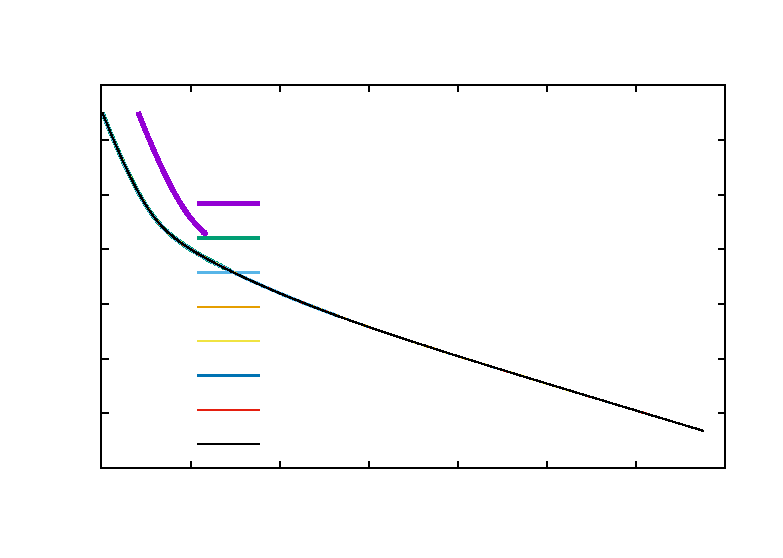
\includegraphics{viscos_rat=10_pos_n_interf}}%
    \gplfronttext
  \end{picture}%
\endgroup
}
        \caption{}
        \label{fig:n_interf_test_pos_film}
      \end{subfigure}
      \caption{Vertical position of the sphere versus time for different numbers of elements used to discretise the interface $N$ for $D = 10$, $\Bo = 1000$ and both (a) $\lambda = 0.1$ and (b) $\lambda = 10$. The curves are identical for all choices of $N \geq 50$. However, the larger the value of $N$ the longer the duration of the simulation.}\label{fig:n_interf_test_pos}
    \end{figure}

Figure~\ref{fig:n_interf_test_vol} shows the effect of $N$ on the time dependence of the volume of upper phase fluid entrained beneath the plane $z = 0$. As with the position curves, these are seen to be independent of $N$ for $N \geq 50$.

    \begin{figure}
      \centering
      \begin{subfigure}[b]{0.5\textwidth}
        \resizebox{\textwidth}{!}{\Large \input{../../Programming/sinking_bim_write_up/trunk/viscos_rat=0_1_vol_n_interf.tex}}
        \caption{}
        \label{fig:n_interf_test_vol_tail}
      \end{subfigure}%
      ~
      \begin{subfigure}[b]{0.5\textwidth}
        \resizebox{\textwidth}{!}{\Large % GNUPLOT: LaTeX picture with Postscript
\begingroup
  \makeatletter
  \providecommand\color[2][]{%
    \GenericError{(gnuplot) \space\space\space\@spaces}{%
      Package color not loaded in conjunction with
      terminal option `colourtext'%
    }{See the gnuplot documentation for explanation.%
    }{Either use 'blacktext' in gnuplot or load the package
      color.sty in LaTeX.}%
    \renewcommand\color[2][]{}%
  }%
  \providecommand\includegraphics[2][]{%
    \GenericError{(gnuplot) \space\space\space\@spaces}{%
      Package graphicx or graphics not loaded%
    }{See the gnuplot documentation for explanation.%
    }{The gnuplot epslatex terminal needs graphicx.sty or graphics.sty.}%
    \renewcommand\includegraphics[2][]{}%
  }%
  \providecommand\rotatebox[2]{#2}%
  \@ifundefined{ifGPcolor}{%
    \newif\ifGPcolor
    \GPcolorfalse
  }{}%
  \@ifundefined{ifGPblacktext}{%
    \newif\ifGPblacktext
    \GPblacktexttrue
  }{}%
  % define a \g@addto@macro without @ in the name:
  \let\gplgaddtomacro\g@addto@macro
  % define empty templates for all commands taking text:
  \gdef\gplbacktext{}%
  \gdef\gplfronttext{}%
  \makeatother
  \ifGPblacktext
    % no textcolor at all
    \def\colorrgb#1{}%
    \def\colorgray#1{}%
  \else
    % gray or color?
    \ifGPcolor
      \def\colorrgb#1{\color[rgb]{#1}}%
      \def\colorgray#1{\color[gray]{#1}}%
      \expandafter\def\csname LTw\endcsname{\color{white}}%
      \expandafter\def\csname LTb\endcsname{\color{black}}%
      \expandafter\def\csname LTa\endcsname{\color{black}}%
      \expandafter\def\csname LT0\endcsname{\color[rgb]{1,0,0}}%
      \expandafter\def\csname LT1\endcsname{\color[rgb]{0,1,0}}%
      \expandafter\def\csname LT2\endcsname{\color[rgb]{0,0,1}}%
      \expandafter\def\csname LT3\endcsname{\color[rgb]{1,0,1}}%
      \expandafter\def\csname LT4\endcsname{\color[rgb]{0,1,1}}%
      \expandafter\def\csname LT5\endcsname{\color[rgb]{1,1,0}}%
      \expandafter\def\csname LT6\endcsname{\color[rgb]{0,0,0}}%
      \expandafter\def\csname LT7\endcsname{\color[rgb]{1,0.3,0}}%
      \expandafter\def\csname LT8\endcsname{\color[rgb]{0.5,0.5,0.5}}%
    \else
      % gray
      \def\colorrgb#1{\color{black}}%
      \def\colorgray#1{\color[gray]{#1}}%
      \expandafter\def\csname LTw\endcsname{\color{white}}%
      \expandafter\def\csname LTb\endcsname{\color{black}}%
      \expandafter\def\csname LTa\endcsname{\color{black}}%
      \expandafter\def\csname LT0\endcsname{\color{black}}%
      \expandafter\def\csname LT1\endcsname{\color{black}}%
      \expandafter\def\csname LT2\endcsname{\color{black}}%
      \expandafter\def\csname LT3\endcsname{\color{black}}%
      \expandafter\def\csname LT4\endcsname{\color{black}}%
      \expandafter\def\csname LT5\endcsname{\color{black}}%
      \expandafter\def\csname LT6\endcsname{\color{black}}%
      \expandafter\def\csname LT7\endcsname{\color{black}}%
      \expandafter\def\csname LT8\endcsname{\color{black}}%
    \fi
  \fi
    \setlength{\unitlength}{0.0500bp}%
    \ifx\gptboxheight\undefined%
      \newlength{\gptboxheight}%
      \newlength{\gptboxwidth}%
      \newsavebox{\gptboxtext}%
    \fi%
    \setlength{\fboxrule}{0.5pt}%
    \setlength{\fboxsep}{1pt}%
\begin{picture}(7200.00,5040.00)%
    \gplgaddtomacro\gplbacktext{%
      \csname LTb\endcsname%
      \put(550,704){\makebox(0,0)[r]{\strut{}$0$}}%
      \put(550,1112){\makebox(0,0)[r]{\strut{}$1$}}%
      \put(550,1521){\makebox(0,0)[r]{\strut{}$2$}}%
      \put(550,1929){\makebox(0,0)[r]{\strut{}$3$}}%
      \put(550,2337){\makebox(0,0)[r]{\strut{}$4$}}%
      \put(550,2746){\makebox(0,0)[r]{\strut{}$5$}}%
      \put(550,3154){\makebox(0,0)[r]{\strut{}$6$}}%
      \put(550,3562){\makebox(0,0)[r]{\strut{}$7$}}%
      \put(550,3971){\makebox(0,0)[r]{\strut{}$8$}}%
      \put(550,4379){\makebox(0,0)[r]{\strut{}$9$}}%
      \put(682,484){\makebox(0,0){\strut{}$-10$}}%
      \put(1556,484){\makebox(0,0){\strut{}$0$}}%
      \put(2431,484){\makebox(0,0){\strut{}$10$}}%
      \put(3305,484){\makebox(0,0){\strut{}$20$}}%
      \put(4180,484){\makebox(0,0){\strut{}$30$}}%
      \put(5054,484){\makebox(0,0){\strut{}$40$}}%
      \put(5929,484){\makebox(0,0){\strut{}$50$}}%
      \put(6803,484){\makebox(0,0){\strut{}$60$}}%
    }%
    \gplgaddtomacro\gplfronttext{%
      \csname LTb\endcsname%
      \put(176,2541){\rotatebox{-270}{\makebox(0,0){\strut{}$V$}}}%
      \put(3742,154){\makebox(0,0){\strut{}$t$}}%
      \put(3742,4709){\makebox(0,0){\strut{}$\lambda = 10$, $D = 10$, $\Bo = 1000$}}%
      \put(5913,3462){\makebox(0,0){\strut{}$N$}}%
      \csname LTb\endcsname%
      \put(5816,3242){\makebox(0,0)[r]{\strut{}50}}%
      \csname LTb\endcsname%
      \put(5816,2912){\makebox(0,0)[r]{\strut{}100}}%
      \csname LTb\endcsname%
      \put(5816,2582){\makebox(0,0)[r]{\strut{}150}}%
      \csname LTb\endcsname%
      \put(5816,2252){\makebox(0,0)[r]{\strut{}200}}%
      \csname LTb\endcsname%
      \put(5816,1922){\makebox(0,0)[r]{\strut{}250}}%
      \csname LTb\endcsname%
      \put(5816,1592){\makebox(0,0)[r]{\strut{}300}}%
      \csname LTb\endcsname%
      \put(5816,1262){\makebox(0,0)[r]{\strut{}350}}%
      \csname LTb\endcsname%
      \put(5816,932){\makebox(0,0)[r]{\strut{}400}}%
    }%
    \gplbacktext
    \put(0,0){\includegraphics{../../Programming/sinking_bim_write_up/trunk/viscos_rat=10_vol_n_interf}}%
    \gplfronttext
  \end{picture}%
\endgroup
}
        \caption{}
        \label{fig:n_interf_test_vol_film}
      \end{subfigure}
      \caption{Volume of upper phase fluid entrained below the plane $z = 0$ as a function of time for different numbers of elements used to discretise the interface $N$ for $D = 10$, $\Bo = 1000$ and both (a) $\lambda = 0.1$ and (b) $\lambda = 10$. The curves are identical for all choices of $N \geq 50$.}\label{fig:n_interf_test_vol}
    \end{figure}

\subsection{Numerical Differentiation of Interface}
\label{subsec:num_diff}

At each timestep it is necessary to differentiate the functions $r(s)$ and $z(s)$ that describe the interface as a function of arc-length (subsection~\ref{subsec:eval_coeff}). The numerical differentiation routines used require the choice of an initial step-size $\Delta s$ \citep{Press07}. The sensitivity of the model to this choice has been investigated and it is shown that results are independent of $\Delta s$ for $\Delta s \leq 0.1$ (figures~\ref{fig:diff_test_pos} and~\ref{fig:diff_test_vol}).
    \begin{figure}
      \centering
      \begin{subfigure}[b]{0.5\textwidth}
        \resizebox{\textwidth}{!}{\Large \input{../../Programming/sinking_bim_write_up/trunk/viscos_rat=0_1_pos_diff.tex}}
        \caption{}
        \label{fig:diff_test_pos_tail}
      \end{subfigure}%
      ~
      \begin{subfigure}[b]{0.5\textwidth}
        \resizebox{\textwidth}{!}{\Large % GNUPLOT: LaTeX picture with Postscript
\begingroup
  \makeatletter
  \providecommand\color[2][]{%
    \GenericError{(gnuplot) \space\space\space\@spaces}{%
      Package color not loaded in conjunction with
      terminal option `colourtext'%
    }{See the gnuplot documentation for explanation.%
    }{Either use 'blacktext' in gnuplot or load the package
      color.sty in LaTeX.}%
    \renewcommand\color[2][]{}%
  }%
  \providecommand\includegraphics[2][]{%
    \GenericError{(gnuplot) \space\space\space\@spaces}{%
      Package graphicx or graphics not loaded%
    }{See the gnuplot documentation for explanation.%
    }{The gnuplot epslatex terminal needs graphicx.sty or graphics.sty.}%
    \renewcommand\includegraphics[2][]{}%
  }%
  \providecommand\rotatebox[2]{#2}%
  \@ifundefined{ifGPcolor}{%
    \newif\ifGPcolor
    \GPcolorfalse
  }{}%
  \@ifundefined{ifGPblacktext}{%
    \newif\ifGPblacktext
    \GPblacktexttrue
  }{}%
  % define a \g@addto@macro without @ in the name:
  \let\gplgaddtomacro\g@addto@macro
  % define empty templates for all commands taking text:
  \gdef\gplbacktext{}%
  \gdef\gplfronttext{}%
  \makeatother
  \ifGPblacktext
    % no textcolor at all
    \def\colorrgb#1{}%
    \def\colorgray#1{}%
  \else
    % gray or color?
    \ifGPcolor
      \def\colorrgb#1{\color[rgb]{#1}}%
      \def\colorgray#1{\color[gray]{#1}}%
      \expandafter\def\csname LTw\endcsname{\color{white}}%
      \expandafter\def\csname LTb\endcsname{\color{black}}%
      \expandafter\def\csname LTa\endcsname{\color{black}}%
      \expandafter\def\csname LT0\endcsname{\color[rgb]{1,0,0}}%
      \expandafter\def\csname LT1\endcsname{\color[rgb]{0,1,0}}%
      \expandafter\def\csname LT2\endcsname{\color[rgb]{0,0,1}}%
      \expandafter\def\csname LT3\endcsname{\color[rgb]{1,0,1}}%
      \expandafter\def\csname LT4\endcsname{\color[rgb]{0,1,1}}%
      \expandafter\def\csname LT5\endcsname{\color[rgb]{1,1,0}}%
      \expandafter\def\csname LT6\endcsname{\color[rgb]{0,0,0}}%
      \expandafter\def\csname LT7\endcsname{\color[rgb]{1,0.3,0}}%
      \expandafter\def\csname LT8\endcsname{\color[rgb]{0.5,0.5,0.5}}%
    \else
      % gray
      \def\colorrgb#1{\color{black}}%
      \def\colorgray#1{\color[gray]{#1}}%
      \expandafter\def\csname LTw\endcsname{\color{white}}%
      \expandafter\def\csname LTb\endcsname{\color{black}}%
      \expandafter\def\csname LTa\endcsname{\color{black}}%
      \expandafter\def\csname LT0\endcsname{\color{black}}%
      \expandafter\def\csname LT1\endcsname{\color{black}}%
      \expandafter\def\csname LT2\endcsname{\color{black}}%
      \expandafter\def\csname LT3\endcsname{\color{black}}%
      \expandafter\def\csname LT4\endcsname{\color{black}}%
      \expandafter\def\csname LT5\endcsname{\color{black}}%
      \expandafter\def\csname LT6\endcsname{\color{black}}%
      \expandafter\def\csname LT7\endcsname{\color{black}}%
      \expandafter\def\csname LT8\endcsname{\color{black}}%
    \fi
  \fi
    \setlength{\unitlength}{0.0500bp}%
    \ifx\gptboxheight\undefined%
      \newlength{\gptboxheight}%
      \newlength{\gptboxwidth}%
      \newsavebox{\gptboxtext}%
    \fi%
    \setlength{\fboxrule}{0.5pt}%
    \setlength{\fboxsep}{1pt}%
\begin{picture}(7200.00,5040.00)%
    \gplgaddtomacro\gplbacktext{%
      \csname LTb\endcsname%
      \put(814,704){\makebox(0,0)[r]{\strut{}$-10$}}%
      \put(814,1163){\makebox(0,0)[r]{\strut{}$-8$}}%
      \put(814,1623){\makebox(0,0)[r]{\strut{}$-6$}}%
      \put(814,2082){\makebox(0,0)[r]{\strut{}$-4$}}%
      \put(814,2542){\makebox(0,0)[r]{\strut{}$-2$}}%
      \put(814,3001){\makebox(0,0)[r]{\strut{}$0$}}%
      \put(814,3460){\makebox(0,0)[r]{\strut{}$2$}}%
      \put(814,3920){\makebox(0,0)[r]{\strut{}$4$}}%
      \put(814,4379){\makebox(0,0)[r]{\strut{}$6$}}%
      \put(946,484){\makebox(0,0){\strut{}$-10$}}%
      \put(1597,484){\makebox(0,0){\strut{}$0$}}%
      \put(2248,484){\makebox(0,0){\strut{}$10$}}%
      \put(2898,484){\makebox(0,0){\strut{}$20$}}%
      \put(3549,484){\makebox(0,0){\strut{}$30$}}%
      \put(4200,484){\makebox(0,0){\strut{}$40$}}%
      \put(4851,484){\makebox(0,0){\strut{}$50$}}%
      \put(5501,484){\makebox(0,0){\strut{}$60$}}%
      \put(6152,484){\makebox(0,0){\strut{}$70$}}%
      \put(6803,484){\makebox(0,0){\strut{}$80$}}%
    }%
    \gplgaddtomacro\gplfronttext{%
      \csname LTb\endcsname%
      \put(176,2541){\rotatebox{-270}{\makebox(0,0){\strut{}$z_{\text{c}}$}}}%
      \put(3874,154){\makebox(0,0){\strut{}$t$}}%
      \put(3874,4709){\makebox(0,0){\strut{}$\lambda = 10$, $D = 10$, $\Bo = 1000$}}%
      \put(1901,3462){\makebox(0,0){\strut{}$\Delta s$}}%
      \csname LTb\endcsname%
      \put(1870,3242){\makebox(0,0)[r]{\strut{}$10^{-7}$}}%
      \csname LTb\endcsname%
      \put(1870,2912){\makebox(0,0)[r]{\strut{}$10^{-6}$}}%
      \csname LTb\endcsname%
      \put(1870,2582){\makebox(0,0)[r]{\strut{}$10^{-5}$}}%
      \csname LTb\endcsname%
      \put(1870,2252){\makebox(0,0)[r]{\strut{}$10^{-4}$}}%
      \csname LTb\endcsname%
      \put(1870,1922){\makebox(0,0)[r]{\strut{}$10^{-3}$}}%
      \csname LTb\endcsname%
      \put(1870,1592){\makebox(0,0)[r]{\strut{}$10^{-2}$}}%
      \csname LTb\endcsname%
      \put(1870,1262){\makebox(0,0)[r]{\strut{}$10^{-1}$}}%
      \csname LTb\endcsname%
      \put(1870,932){\makebox(0,0)[r]{\strut{}$10^{0}$}}%
    }%
    \gplbacktext
    \put(0,0){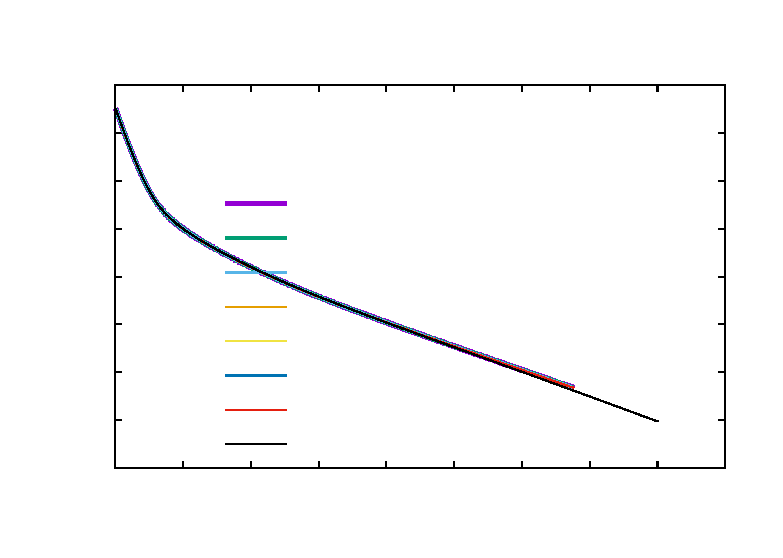
\includegraphics{viscos_rat=10_pos_diff}}%
    \gplfronttext
  \end{picture}%
\endgroup
}
        \caption{}
        \label{fig:diff_test_pos_film}
      \end{subfigure}
      \caption{Vertical position of the sphere versus time for different values of the initial step size for numerical differentiation for $D = 10$, $\Bo = 1000$ and both (a) $\lambda = 0.1$ and (b) $\lambda = 10$. The curves are identical for all choices of $\Delta s \leq 0.1$.}\label{fig:diff_test_pos}
    \end{figure}


    \begin{figure}
      \centering
      \begin{subfigure}[b]{0.5\textwidth}
        \resizebox{\textwidth}{!}{\Large \input{../../Programming/sinking_bim_write_up/trunk/viscos_rat=0_1_vol_diff.tex}}
        \caption{}
        \label{fig:diff_test_vol_tail}
      \end{subfigure}%
      ~
      \begin{subfigure}[b]{0.5\textwidth}
        \resizebox{\textwidth}{!}{\Large \input{../../Programming/sinking_bim_write_up/trunk/viscos_rat=10_vol_diff.tex}}
        \caption{}
        \label{fig:diff_test_vol_film}
      \end{subfigure}
      \caption{Time dependence of volume of upper phase fluid entrained below the plane $z = 0$ for different values of the initial step size for numerical differentiation for $D = 10$, $\Bo = 1000$ and both (a) $\lambda = 0.1$ and (b) $\lambda = 10$. The curves are identical for all choices of $\Delta s \leq 0.1$.}\label{fig:diff_test_vol}
    \end{figure}

\subsection{Experimental Verification}
\label{subsec:exp_verif}


